\documentclass[a4paper,9pt]{report}
\usepackage[margin=2.5cm]{geometry}
\usepackage{graphicx}
\usepackage{fancyhdr}
\usepackage{hyperref}
\usepackage{tikz}
\usepackage{lipsum} % For filler text if needed
\usepackage{setspace}
\usepackage{titlesec}
\usepackage{everypage}
\usepackage{caption}
\usepackage{subcaption}
\usepackage{amsmath}
\usepackage{amsfonts} % For \mathbb{R} and other mathematical symbols
\usepackage{comment}
\usepackage{xcolor}
\usepackage{booktabs}
\usepackage{float} % For [H] placement option
% --- No page numbering for title ---
\pagestyle{fancy}
\fancyhf{}
\setlength{\footskip}{56.99039pt}
\fancyfoot[C]{\thepage}
\definecolor{darkgreen}{RGB}{0,100,0}
\definecolor{myorange}{RGB}{255,165,0}
% --- Bottom-right logo ---
\fancyfoot[R]{
    \raisebox{0.1\textwidth}{
\includegraphics[height=0.25cm]{ressources/for_glory.png}}
}
\begin{document}

% --- Logo Placement with TikZ ---
\begin{tikzpicture}[remember picture, overlay]
    % Top-left: Company Logo
    \node[anchor=north west, xshift=1cm, yshift=-3cm] at (current page.north west) {
        
\includegraphics[width=0.5\textwidth, keepaspectratio]{ressources/ss_horizontal_white_on_black.jpg}
    };

    % Top-right: University Logo
    \node[anchor=north east, xshift=-1cm, yshift=-2cm] at (current page.north east) {
        
\includegraphics[width=0.5\textwidth, keepaspectratio]{ressources/logo_upssitech.png}
    };
\end{tikzpicture}

% ------------------------------------------------------------
\vspace*{4cm}

\begin{center}
    \Huge \textbf{Neural-Assisted Feature Matching}\\[1.5cm]
    \LARGE Internship Report\\[1.5cm]
    \large \textbf{Author:} EL OUARRAT Haytam\\
    \textbf{Internship Period:} Mars – August 2025\\
    \textbf{Location:} SteelSeries, Lille, France\\[2cm]

    \textbf{Advisors:} Pierre Biret, Damien Granger, Raphaël Greff\\
    \textbf{University Supervisor:} Phillipe Joly \\[2cm]

    \large Engineering Degree in Robotics and Interactive Systems \\
    UPSSITECH \\
    University of Toulouse
\end{center}

\vfill

\begin{center}
    \today
\end{center}

% --- Page Break 
\newpage
\begin{abstract}
    Real-time analysis of gaming footage requires feature matching algorithms that are both robust and computationally efficient. SteelSeries’ Moments software currently relies on the Scale-Invariant Feature Transform (SIFT) to detect and match in-game icons, offering strong invariance to scale, rotation, and illumination changes. However, SIFT’s high computational cost and latency make it unsuitable for high frame rate, CPU-bound environments. This work proposes a Neural-Assisted Feature Matching approach that accelerates the most computationally intensive stages of SIFT—keypoint detection and descriptor computation—through the integration of lightweight convolutional neural networks. We investigate recent neural methods, including ALIKE, LightGlue, and XFeat, identifying XFeat as the primary candidate for its favorable speed–accuracy trade-off. A custom gaming-focused dataset was created using real gameplay footage and synthetic transformations to evaluate matching quality, latency, and resource usage. The proposed hybrid pipeline achieves substantial reductions in processing time compared to the existing SIFT-based implementation, while preserving comparable matching accuracy and robustness under varied gaming conditions. These findings demonstrate the potential of neural-assisted methods for real-time, resource-constrained computer vision tasks, with direct applicability to gaming analytics and broader real-time visual correspondence applications.
\end{abstract}

\tableofcontents
\listoffigures
% ------------------------------------------------------------
\chapter{Acknowledgements}
% ------------------------------------------------------------
\chapter{Introduction}

\section{Host Organism}
\subsection{SteelSeries}
\subsubsection{Company history and Background}
Steel\textbf{series}, a Danish manufacturer of gaming peripherals, was founded in 2001 by Jacob Wolff-Petersen. The company originally launched under the name Soft Trading, and made its mark with innovative gaming mousepads in the early 2000s. In 2007, Soft Trading rebranded to SteelSeries, reflecting its broadened focus beyond mousepads and into a full range of PC gaming accessories. Key milestones in SteelSeries' evolution include the 2008 acquisition of Ideazon, which brought the Zboard and World of Warcraft gaming keyboard into its portfolio and furthered its presence in the North American market.
The company grew rapidly in the 2010s, fueled by its involvement in the esports scene and partnerships with professional gamers. SteelSeries has since expanded its product line to include high-performance gaming mice, keyboards, headsets, and mousepads, becoming a leading brand in the gaming industry.

\subsubsection{Key Products and Technologies}
SteelSeries, renowned for its gaming peripherals and accessories, spanning several product categories. Its product portfolio includes:
\begin{itemize}
    \item \textbf{Gaming Mice:} High-precision mice with customizable buttons and sensors.
    \begin{figure}[h!]
    \centering
    \begin{subfigure}[b]{0.25\textwidth}
        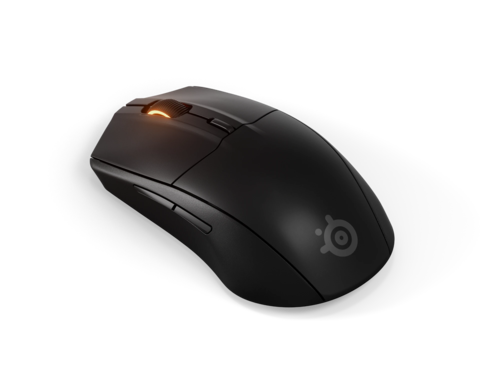
\includegraphics[width=\textwidth]{ressources/mouse_1.png}
        \caption{Rival 3 Wireless Gen 2}
    \end{subfigure}
    \hfill
    \begin{subfigure}[b]{0.25\textwidth}
        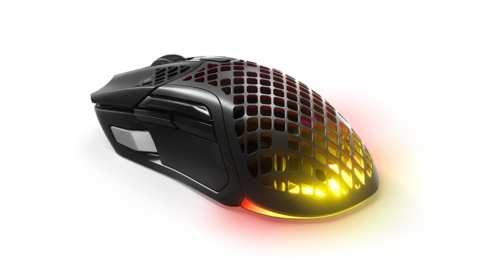
\includegraphics[width=\textwidth]{ressources/mouse_2.png}
        \caption{Aerox 5}
    \end{subfigure}
    \hfill
    \begin{subfigure}[b]{0.25\textwidth}
        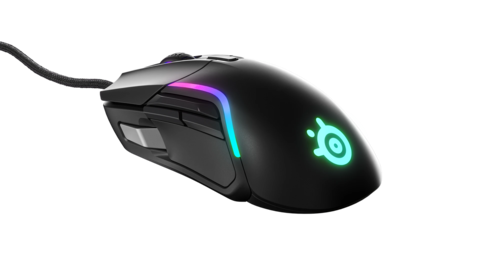
\includegraphics[width=\textwidth]{ressources/mouse_3.png}
        \caption{Rival 5}
    \end{subfigure}
    \caption{SteelSeries Gaming Mice}
    \end{figure}
    \item \textbf{Keyboards:} Mechanical and membrane keyboards designed for gaming performance.
    \begin{figure}[h!]
    \centering
    \begin{subfigure}[b]{0.25\textwidth}
        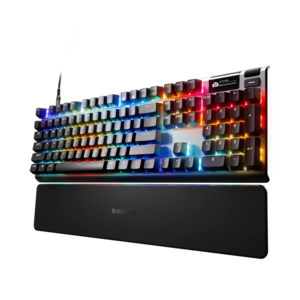
\includegraphics[width=\textwidth]{ressources/kb_1.png}
        \caption{Apex Pro Gen 3}
    \end{subfigure}
    \hfill
    \begin{subfigure}[b]{0.25\textwidth}
        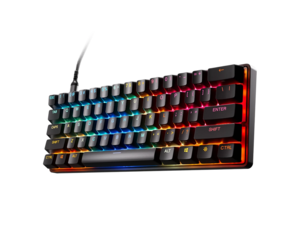
\includegraphics[width=\textwidth]{ressources/kb_2.png}
        \caption{Apex Pro Mini Gen 3}
    \end{subfigure}
    \hfill
    \begin{subfigure}[b]{0.25\textwidth}
        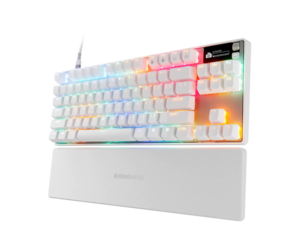
\includegraphics[width=\textwidth]{ressources/kb_3.png}
        \caption{Apex Pro TKL Gen 3}
    \end{subfigure}
    \caption{SteelSeries Gaming Keyboards}
    \end{figure}
    \item \textbf{Headsets:} Wired and wireless headsets with advanced audio features.
    \begin{figure}[h!]
    \centering
    \begin{subfigure}[b]{0.25\textwidth}
        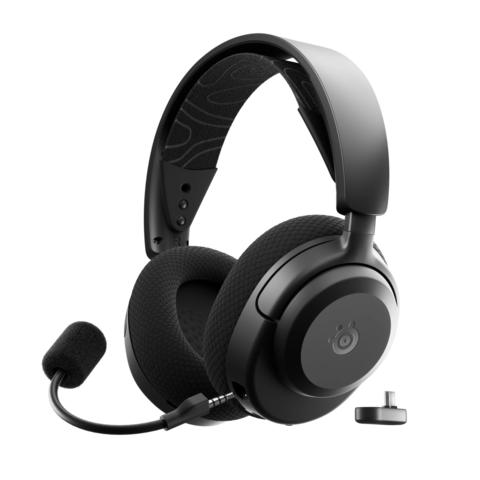
\includegraphics[width=\textwidth]{ressources/hs_2.png}
        \caption{Arctis Nova 3 Wireless}
    \end{subfigure}
    \hfill
    \begin{subfigure}[b]{0.25\textwidth}
        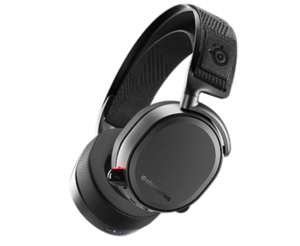
\includegraphics[width=\textwidth]{ressources/hs_3.png}
        \caption{Arctis Pro Wireless}
    \end{subfigure}
    \hfill
    \begin{subfigure}[b]{0.25\textwidth}
        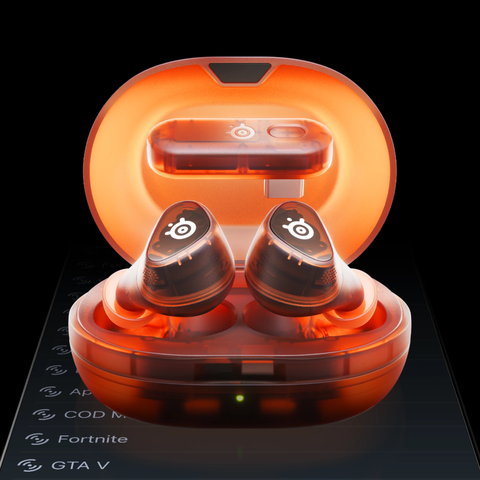
\includegraphics[width=\textwidth]{ressources/hs_1.png}
        \caption{Arctis GameBuds™ Glorange}
    \end{subfigure}
    \caption{SteelSeries Gaming Keyboards}
    \end{figure}
    \item \textbf{Mousepads:} Various sizes and materials optimized for different play styles.
    \item \textbf{Software:}
        \begin{itemize}
        \item \textbf{SteelSeries GG:} is an all-in-one software platform that brings together the various tools and services SteelSeries offers to enhance the gaming experience. It serves as the central hub for managing SteelSeries peripherals and includes multiple sub-applications.
        \item \textbf{SteelSeries Engine:} the part of GG that handles the core device configuration. It's used to customize settings for SteelSeries mice, keyboards, headsets, and other gear. Through Engine, users can adjust RGB lighting effects, set up macros, and fine-tune mouse sensitivity (DPI).
        \item SteelSeries' advanced audio suite built specifically for gamers who want precise control over their sound experience. It offers a powerful parametric equalizer that lets users independently customize audio for game sounds, voice chat, and microphone input.
        \item \textbf{SteelSeries Moments:} a gameplay capture tool within GG that automatically records key moments during gaming sessions. It can detect in-game events like kills, wins, or goals and save short clips around those events.
        \end{itemize} 
\end{itemize}

\subsection{Mission}
SteelSeries' mission is to create the best gaming gear in the world, empowering gamers to perform at their best, whether it is for professionals who seek perfection, or casuals who seek a sense of competition and completion. Its implication over the years in the esports scene has made it a trusted brand among professional gamers, and its commitment to innovation continues to drive the development of new products that enhance the gaming experience. Most notably, SKT Gaming, a professional esports organization, has been using SteelSeries products since 2012, and has won multiple championships in games like CS:GO and League of Legends etc.
\begin{figure}[H]
    \centering
    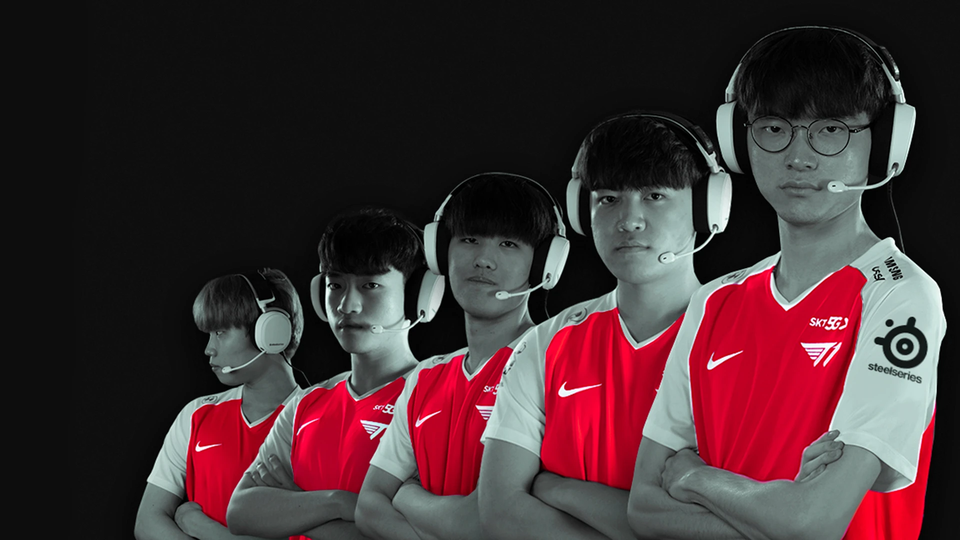
\includegraphics[width=0.7\textwidth]{ressources/sktt1.png}
    \caption{5x League of Legends World Champions SKT T1}
    \label{fig:5x League of Legends World Champions SKT T1}
\end{figure}
\section{Context \& Motivation}
\subsection{SteelSeries’s Objective}
SteelSeries software, and particularly the \textit{Moments} application, is designed to run alongside demanding video games without interrupting or degrading the user’s experience. To achieve this, the software must be able to detect the appearance of predefined visual templates within the live feed of the player, such as icons or achievement indicators, in order to automatically capture highlights. This task requires a feature matching method that is:

\begin{itemize}
    \item \textbf{Fast:} able to process frames in real time with minimal latency so as not to interfere with the game’s performance.
    \item \textbf{Reliable:} consistently functional across different games, visual styles, and in-game conditions.
    \item \textbf{Accurate:} capable of pinpointing the presence and location of the template without producing false detections.
\end{itemize}

The core objective for SteelSeries, therefore, is to employ a feature matching solution that balances these requirements, ensuring smooth integration with gaming sessions and maintaining the performance expectations of competitive and casual players alike.

\subsection{Feature Matching in Computer Vision}
\subsubsection{Definition}
Feature matching refers to the process of finding corresponding keypoints between two images of the same scene or object. These keypoints are distinctive image features, such as corners, edges, blobs, or regions with significant intensity changes that can be reliably identified in different images, even if those images have undergone transformations.
\subsection{How Feature Matching Works}
Feature matching typically involves several steps:
\begin{itemize}
    \item \textbf{Feature Extraction:} the initial step in feature matching, identifies distinctive, stable, and informative points of high-intensity variation—such as corners or edges—that are invariant to changes in rotation and scale.
    \item \textbf{Feature Description:} the process of computing a descriptor for each keypoint, which is a compact representation of the local image patch around the keypoint. This descriptor should be robust to changes in lighting, viewpoint, and other image transformations.
    \item \textbf{Feature Matching:} the final step involves finding correspondences between the keypoints in the two images based on their descriptors. This is typically done using techniques like nearest neighbor search, where the descriptor of each keypoint in one image is compared to all descriptors in the other image to find the best match.
\end{itemize}
\subsection{Scale Invariant Feature Transform}
In David G. Lowe’s 2004 paper, \textbf{SIFT} stands for \textit{Scale Invariant Feature Transform}, a method designed to detect and describe local features in images that remain stable across various transformations. The term encapsulates the core strengths of the algorithm:
\begin{itemize}
    \item \textbf{Scale Invariance:} SIFT demonstrates robustness against changes in image size by detecting extrema in scale-space using a Difference-of-Gaussian approach, making it effective across different zoom levels and image resolutions.
    
    \item \textbf{Transformation Resilience:} The algorithm maintains stability under various image transformations including rotation, scaling, partial changes in illumination, and viewpoint variations, ensuring reliable feature detection across different viewing conditions.
    
    \item \textbf{Distinctive Feature Representation:} SIFT identifies keypoints characterized by location, scale, orientation, and descriptor vectors based on local gradients, converting raw image data into a highly distinctive representation suitable for matching and recognition tasks.
\end{itemize}
Thus, SIFT provides a powerful framework for extracting and matching image features under challenging real-world conditions~\cite{lowe2004}.

\subsection{Challenges in Gaming Applications}
The primary challenge for image processing in real-time gaming is the extreme demand for \textbf{speed} and \textbf{low latency}, as any analysis must occur within a tight millisecond timeframe to avoid introducing lag. This becomes particularly difficult because image processing algorithms must \textit{compete for the same computational resources} that the game itself is using. This is not a minor issue, as modern AAA titles are specifically designed to \textbf{monopolize the GPU}. Games like \textit{Alan Wake 2} or \textit{Cyberpunk 2077}, with demanding features such as \textit{path tracing}, already push high-end graphics cards to their absolute limits merely to render the game world. Adding an additional workload like real-time image processing on top of this creates a severe \textbf{performance bottleneck}, forcing developers to make significant trade-offs between \textbf{accuracy} and \textbf{efficiency}, and to rely on \textit{incredibly lightweight algorithms} that won't cripple the game's frame rate.

\subsection{Limitations of Traditional Feature Matching Techniques}
Real-time applications, such as visual odometry (VO), SLAM, and gaming, require both high accuracy and extremely low latency; thus, feature matching algorithms must satisfy very stringent constraints. Traditional feature-based systems using SIFT or ORB work well for reliable and accurate matching under varying conditions, but they are slower because of the explicit data association steps involved. Such latency, however, is unacceptable when one has to make decisions within milliseconds. Zhao and Vela (2020) characterize this trade-off by stating, ``feature-based systems exhibit good performance, yet have higher latency due to explicit data association; direct \& semidirect systems have lower latency, but are inapplicable in some target scenarios or exhibit lower accuracy than feature-based ones''~\cite{zhao2020good}. This observation thus attests the traditional pipelines' readymade opposing factors-speed versus precision-while promoting lightweight or neural-assisted alternatives to ensure on-time delivery without siding with robustness.

\section{Project Objectives}
\subsection{Reproducing Feature Matching Techniques with Neural Networks}
Recent years have witnessed a surge of interest in leveraging neural networks to enhance image processing tasks, applications in this field range from image classification and object detection to semantic segmentation and vision language models. The idea is to use neural networks to learn the feature extraction and matching process, potentially leading to faster and more efficient algorithms. This project aims to explore the feasibility of using neural networks to reproduce traditional feature matching techniques, such as SIFT or ORB, while maintaining or improving their performance.
\subsection{Problem Statement}
This research investigates whether lightweight neural networks can effectively accelerate the most computationally intensive stages of traditional feature matching—specifically, keypoint detection and description, in SteelSeries Moments software. By integrating neural-assisted processing into a SIFT-based pipeline, the project aims to achieve substantial reductions in processing time without sacrificing matching accuracy or robustness. The findings will inform not only gaming software optimization but also the broader application of neural-accelerated methods in real-time computer vision, particularly on hardware-limited platforms.
\section{Industrial Relevance}
\subsection{Integration with SteelSeries Moments Software}
For a company like SteelSeries, which leads in the gaming and esports market, user experience is paramount. The primary goal of this project is to achieve a reduced processing time compared to the traditional SIFT method, currently in-use in the SteelSeries Moments software. This will allow users to quickly and efficiently analyze their gaming footage, enhancing their overall experience with the product without relying on heavy computational resources.

% ------------------------------------------------------------
\chapter{Literature Review: Neural Feature Matching}
\section{Review of Recent Methods}
In the last decade, neural networks have profoundly reshaped the landscape of
feature matching in all vision tasks, progressively replacing or complementing
traditional methods such as SIFT and ORB. Driven by the relentless pursuit of
computational efficiency, accuracy and adaptability, researches have turned to
deep learning as the logical solution to this challenge, leveraging its
powerful representation-learning capabilities to address longstanding issues in
classicals methods. particularly in fields demanding fast accurate processing,
such as robotics and augmented reality.

\section{ALIKE: Accurate and Lightweight Keypoint Detection and Descriptor Extraction}
To address the issue that existing keypoint detectors are non-differentiable
and cannot be optimized via back-propagation, this paper presents a novel,
partially differentiable keypoint detection module that outputs accurate
sub-pixel keypoints. The method uses a reprojection loss to directly optimize
these keypoints and a dispersity peak loss for regularization, ensuring
accuracy. Descriptors are also extracted at a sub-pixel level, trained with a
stable neural reprojection error loss. This entire process is handled by a
lightweight network capable of running at 95 frames per second on 640x480
images. The proposed method achieves performance equivalent to state-of-the-art
approaches in homography estimation, camera pose estimation, and visual
localization, while significantly reducing inference time.
\begin{figure}[h]
    \centering
    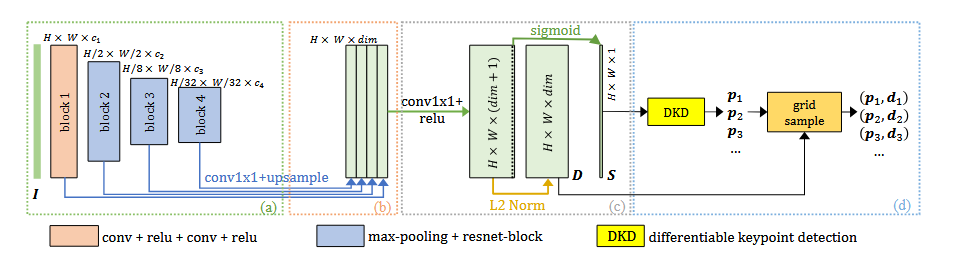
\includegraphics[width=\textwidth]{ressources/alike.png}
    \caption{architecture overview of ALIKE}
    \label{fig:alike}
\end{figure}
\subsection{Shared Feature Encoder}
At its base, ALIKE uses a lightweight Convolutional Neural Network (CNN) as its
backbone. This encoder takes an input image and processes it through several
convolutional layers to produce a set of shared feature maps. This design is
efficient because the computationally intensive process of feature extraction
is done only once, and the results are used for both the detection and
description tasks that follow. The focus is on creating a compact yet powerful
network that can run quickly on standard hardware.
\subsection{Keypoint Detection Head}
This is where ALIKE's main innovation lies. Instead of just identifying pixels
on a grid, the detection head is designed to find keypoints with sub-pixel
accuracy.
\begin{itemize}
    \item \textbf{Score Map Generation:} The detection head first produces a reliability or score map, where high values indicate a higher probability of a keypoint being present.
    \item \textbf{Partially Differentiable Detection:} To achieve sub-pixel accuracy, ALIKE performs a soft-argmax operation on local 2x2 patches of the score map. This process is "partially differentiable," meaning it allows the network to learn the precise location of a keypoint within a pixel's boundaries through back-propagation during training.
    \item \textbf{Loss Functions:} The detection process is optimized using two specific loss functions mentioned in the research:
          \begin{itemize}
              \item \textbf{Reprojection Loss:} This loss directly optimizes the sub-pixel coordinates of the keypoints, pushing them to be more geometrically consistent between different views of the same scene.
                    \begin{equation*}
                        \mathcal{L}_{\text{rep}} = \frac{1}{N} \sum_{i=1}^{N} \left\| p_i - \hat{p}_i \right\|_2
                    \end{equation*}
                    {\footnotesize
                    \begin{description}
                        \item[$\mathcal{L}_{\text{rep}}$] The Reprojection Loss value.
                        \item[$N$] The total number of matching keypoint pairs.
                        \item[$p_i$] The coordinates of a keypoint in the first image.
                        \item[$\hat{p}_i$] The coordinates of the corresponding keypoint from the second image, projected onto the first.
                        \item[$\left\| \cdot \right\|_2$] The L2 norm, which calculates the Euclidean distance between the two points.
                    \end{description}}
              \item \textbf{Dispersity Peak Loss:} This acts as a regularizer, encouraging the score map to have sharp, distinct peaks. This prevents keypoints from clumping together and ensures they are well-defined.
                    \begin{equation*}
                        \mathcal{L}_{\text{peak}} = \frac{1}{W \times H} \sum_{x,y} \left( \max(0, S(x,y) - \max_{\substack{dx,dy \in \{-1,0,1\}^2 \\ (dx,dy) \neq (0,0)}} S(x+dx, y+dy)) \right)
                    \end{equation*}
                    {\footnotesize
                    \begin{description}
                        \item[$\mathcal{L}_{\text{peak}}$] The Dispersity Peak Loss value.
                        \item[$W, H$] The width and height of the score map.
                        \item[$S(x,y)$] The score of the pixel at coordinate $(x,y)$.
                        \item[$\max_{\dots}$] The maximum score found within the 8-pixel neighborhood around the pixel $(x,y)$.
                        \item[$\max(0, \cdot)$] A rectifier (ReLU) ensuring the loss is non-negative. It penalizes pixels that are not a strict local maximum.
                    \end{description}}
          \end{itemize}
\end{itemize}
\subsection{Descriptor Extraction Head}
The descriptor head uses the shared feature maps from the encoder to generate a
distinctive descriptor for each detected keypoint.
\begin{itemize}
    \item \textbf{Sub-Pixel Descriptor Extraction:} To match the precision of the detection head, descriptors are also extracted in a sub-pixel manner. The network uses the precise sub-pixel coordinates generated by the detection head to sample from the descriptor feature map using bilinear interpolation. This ensures that the descriptor accurately represents the feature at its exact location, rather than just the nearest pixel center.
    \item \textbf{Training loss:} The descriptors are trained using a stable neural reprojection error loss. This loss function helps in learning descriptors that are robust to viewpoint and illumination changes, leading to more reliable matching.
\end{itemize}
By combining an efficient backbone with a novel, differentiable method for sub-pixel keypoint detection and description, ALIKE achieves state-of-the-art performance on various matching tasks while maintaining a very high processing speed (e.g., 95 FPS on 640x480 images).
\section{LightGlue: Local Feature Matching at Light Speed}
LightGlue is a deep neural network designed to efficiently and accurately match
local features between images. It builds upon the SuperGlue architecture by
introducing simpler, more efficient design choices that make it faster, more
memory-efficient, easier to train, and adaptive to the complexity of the image
pair. This adaptability allows LightGlue to process easier image pairs more
quickly, making it ideal for time-sensitive tasks like 3D reconstruction. The
model and its training code are publicly available.
\begin{figure}[h]
    \centering
    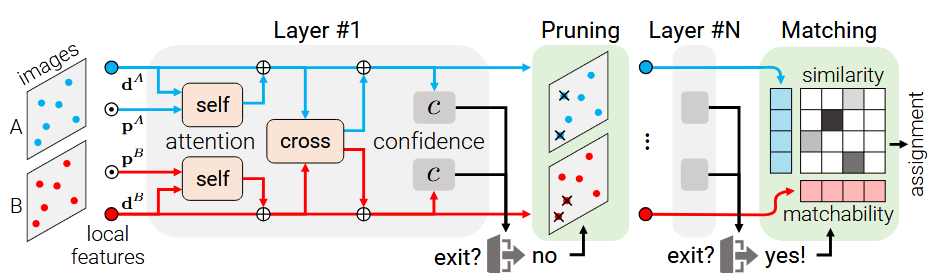
\includegraphics[width=\textwidth]{ressources/lightglue.png}
    \caption{architecture overview of LightGlue}
    \label{fig:lightglue}
\end{figure}
The architecture of LightGlue is designed to match sparse local features between two images efficiently while maintaining high accuracy. It builds upon the SuperGlue framework but introduces several key improvements that make it faster, easier to train, and more adaptive. Here's a breakdown of its core architectural components:
\subsection{Input Representation:}
LightGlue takes as input two sets of local features from both reference and
target image, each feature consists of normalized 2D coordinates and a
256-dimensional descriptor.
\subsection{Transformer-based Backbone: }
LightGlue uses a stack of Transformer layers to jointly process the features
from both images. Each layer includes:
\begin{itemize}
    \item \textbf{Self-Attention Mechanism:} This allows the model to capture long-range dependencies and relationships between features within each image.
    \item \textbf{Cross-Attention Mechanism:} This enables the model to learn correspondences between features from the reference and target images, enhancing the matching process.
\end{itemize}
\subsection{Lightweight Matching Head:}
After each layer, the network can predict similarity scores for all feature
pairs, as well as predict the matchability scores for each point (i.e., whether
a point is likely to have a corresponding point in the other image). It
combines similarity and matchability into a soft partial assignment matrix.
\subsection{Adaptive Inference:}
This is a unique feature of LightGlue, teh ability to dynamically adjust the
computations by using:
\begin{itemize}
    \item \textbf{Adaptive Depth: }after each layer, a classifier predicts if a sufficient number of features
    \item \textbf{Adaptive Depth:} the points predicted as confidently unmatchable are pruned from further processing, reducing computational load.
\end{itemize}
\section{XFeat: Accelerated Features for Lightweight Image Matching}
This work presents a new lightweight CNN structure that redefines the trade-off
between efficiency and accuracy for local feature extraction. In contrast to
existing deep models that need GPUs and/or hardware-specific tuning, XFeat
offers real-time performance on CPU-only systems by combining three components:
a featherweight backbone, a very light keypoint detection branch, and a match
refinement module that was new in its design. XFeat also uniquely has both
sparse and semi-dense matching modes, the first efficient model to do so, and
is suitable for visual localization and pose estimation. XFeat is typically
5–9× faster than other state-of-the-art methods, but offers similar or better
accuracy. The three design choices: growth of channel number tripled, early
resolution preservation, and course-to-fine refinement, contribute to high
quality matching for practical device constraints. It is a scalable,
lightweight and practical deep learning architecture for the real world.
\subsection{Featherweight Network Backbone}
The backbone of XFeat is designed to balance out computational efficiency and
representational accuracy:
\begin{itemize}
    \item \textbf{Channel Distribution Strategy}: The network begins with a minimal number of channels in the initial convolutional layers, where the spatial resolution is highest, to reduce computational load. As the spatial resolution decreases through subsequent layers, the number of channels is increased, following a tripling strategy (e.g starting with 4 channels and increasing up to 128 channels). This approach ensures that the network remains lightweight without compromising on feature extraction quality.
    \item \textbf{Convolutional Blocks}: The architecture comprises six convolutional blocks, each consisting of basic layers that include 2D convolutions  with kernel sizes ranging from 1 to 3, followed by ReLU activations and Batch Normalization. Strides of 2 are used for downsampling, \textbf{progressively reducing the spatial dimensions while increasing the depth of feature maps}
\end{itemize}
\subsection{Local Feature extraction}
XFeat employs specialized heads for different aspects of feature extraction:
\begin{itemize}
    \item \textbf{Descriptors Head}: This component extracts a dense feature map by merging multi-scale features from the encoder using a feature pyramid strategy. Intermediate representations at different scales (1/8, 1/16, and 1/32 of the original resolution) are upsampled and combined to enhance the receptive field without significantly increasing computational demands. A fusion block integrates these representations into the final feature map and an additional convolutional block generates a reliability map that indicates the confidence of each local feature.
    \item \textbf{Keypoint Head}: To efficiently detect keypoints, XFeat introduces a dedicated parallel branch focused on low-level image structures. The input image is represented as a 2D grid of 8x8 pixel  cells, each reshaped into 64-dimensional features. This representation preserves spatial granularity within individual cells while allowing rapid 1x1 convolutions for keypoint regression. After four convolutional layers, a keypoint embedding is obtained, encoding the distribution of keypoints within each cell.
\end{itemize}
\subsection{Dense Matching and Match Refinement}
XFeat includes a lightweight module for dense feature matching:
\begin{itemize}
    \item Match Refinement Module: This module refines coarse matches to achieve
          pixel-level accuracy without requiring high-resolution feature maps. It employs
          a simple MLP (Multi-Layer Perceptron), that predicts offsets between matching
          features, enabling efficient semi-dense matching suitable for
          resource-constrained settings.
\end{itemize}
\subsubsection{What is Mutual Nearest Neighbor?}
MNN, is a popular matching strategy used in image correspondence tasks to
robustly establish matches between two sets of local feature descriptors. It
helps ensure that matches are reciprocal, which greatly reduces false matches
compared to simple nearest neighbor methods. \subsubsection*{Mutual Nearest
    Neighbors (MNN) Algorithm}
\begin{itemize}
    \item \textbf{Compute Nearest Neighbors}: Given two feature sets:
          \begin{itemize}
              \item Set $A = \{a_1, a_2, \ldots, a_n\}$
              \item Set $B = \{b_1, b_2, \ldots, b_m\}$
          \end{itemize}
          For each feature $a_i \in A$, find its nearest neighbor in $B$ using:
          \[
              \text{NN}(a_i, B) = \arg\min_{b_j \in B} \|a_i - b_j\|
          \]
          where $\| \cdot \|$ is the Euclidean distance metric.
    \item \textbf{Reciprocal Check}
          For each candidate pair $(a_i, b_j)$ from Step 1:
          \begin{enumerate}
              \item Verify mutual nearest neighbor relationship:
                    \begin{align*}
                        \text{NN}(a_i, B) & = b_j \quad \text{(Original condition from Step 1)} \\
                        \text{NN}(b_j, A) & = a_i \quad \text{(Reciprocal condition)}
                    \end{align*}
              \item The pair $(a_i, b_j)$ is considered valid MNN iff both conditions hold [2][5]
          \end{enumerate}
    \item \textbf{Formal Definition}
          A pair $(a_i, b_j)$ is mutual nearest neighbors if:
          \[
              \forall b_k \in B, \|a_i - b_j\| \leq \|a_i - b_k\| \quad \land \quad \forall a_l \in A, \|b_j - a_i\| \leq \|b_j - a_l\|
          \]
          This bidirectional verification ensures correspondence stability in feature
          matching applications.
    \item \textbf{Discard Non-mutual Matches}
          If a pair does not fulfill mutual nearest neighbor criteria, it is discarded.
          After discarding non-mutual pairs, the final matched pairs are most robust against ambiguous matches.
\end{itemize}
\subsection{Sparse \& Semi-dense Matching}
The paper introduces two different matching modes based on previously explained
MNN, \textit{XFeat} and \textit{XFeat*}, they differ in the way they carry
image matching: \\

{\footnotesize
\begin{tabular}{|l|l|l|}
    \hline
    Aspect                & XFeat                                        & XFeat* (Star)                                \\
    \hline
    Matching strategy     & Sparse matching (keypoint-based)             & Semi-dense matching (coarse feature maps)    \\
    \hline
    Keypoints used        & Small set (up to 4,096 typically)            & Larger set (~10,000 typically)               \\
    \hline
    Refinement step       & No refinement                                & Match refinement (coarse-to-fine)            \\
    \hline
    Accuracy              & Good                                         & Higher (due to dense matching \& refinement) \\
    \hline
    Computational Cost    & Lower (faster, simpler)                      & Slightly higher (but still lightweight)      \\
    \hline
    Application scenarios & Visual localization, fast real-time matching & Pose estimation, dense scene                 \\
    \hline
\end{tabular}
}
\begin{enumerate}
    \item Sparse (XFeat) vs. Semi-dense Matching (XFeat*):
          \begin{itemize}
              \item \textit{XFeat} extracts a small set of keypoints (defaulting to 4096), uses Mutual Nearest Neighbor to match sparse features. It is fast and suitable for applications that prioritize speed and simplicity, such as visual localization or robotics.
              \item \textit{XFeat*} extracts semi-dense features, typically around 10,000 descriptors, and retains descriptors densely at different scales. It also performs matching in a coarse-to-fine manner, capturing more detailed correspondences across the image.
          \end{itemize}
    \item Match Refinement in \textit{XFeat*}: \\ XFeat* introduces a lightweight match
          refinement module: \\ Matches descriptors at a coarse level first. Then
          predicts pixel-level offsets to refine matches to exact pixel coordinates. This
          refinement significantly improves accuracy, especially in scenarios demanding
          precise correspondences (e.g., detailed scene reconstruction). \textit{XFeat}
          on the other hand has no such refinement; matches are at the original, coarse
          level.
    \item To resume: \\ {\footnotesize
          \begin{tabular}{|l|l|l|}
              \hline
              Metric             & XFeat (Basic) & XFeat* (Star)                            \\
              \hline
              Speed              & Very Fast     & Fast (slightly slower due to refinement) \\
              \hline
              Accuracy           & Good          & Higher accuracy                          \\
              \hline
              Density of matches & Sparse        & Semi-dense                               \\
              \hline
              Robustness         & Robust        & More robust                              \\
              \hline
          \end{tabular}
          }
          \begin{itemize}
              \item \textit{XFeat} is a fast, sparse matching approach focusing on extreme computational efficiency.
              \item \textit{XFeat*} is a semi-dense, refined matching approach, offering better accuracy at the slight expense of computational resources.
          \end{itemize}
\end{enumerate}
\section{Gaps and Limitations}
While there have been substantial advancements in neural-supported feature matching, frameworks such as ALIKE, XFeat, and LightGlue each encounter trade-offs limiting their suitability for purpose-built 2D image contexts. ALIKE does a great job at efficient keypoint detection and binary descriptors which makes it suitable for mobile and embedded contexts, but it is limited as it provides no built-in matching pipeline, and poor detection performance when the stimulus contains low-texture or synthetic scenarios, such as gaming or icon-based imagery. LightGlue employs an attention-based transformer model that makes it robust to perspective and lighting changes, but this comes at a high computational cost that also limits its adaptability to low-cost or low-latency environments for rapid feature matching. This state of play lays bare a glaring gap in the research alignment: there is no single feature matching framework that combines the benefit of speed (e.g., ALIKE and XFeat) with the ability to adaptively and robustly handle image distortion to the extent of (or more) than LightGlue, and is specifically optimized for "2D" applications, such as icon localization, synthetic-to-real matching, and dynamic in-game overlays—where conventional 3D priors and richly textured cues are often absent or unreliable. XFeat improves upon some its limitations by adopting a more integrated process to detection, description, and matching in a lightweight end-to-end model that demonstrates impressive efficiency gains when doing computationally expensive matching comparisons, however, its performance is limited when considering view and lighting changes or changing imagery states when the model is representative of highly structured and realistic 2D datasets.

% ------------------------------------------------------------
\chapter{Methodology}
\section{Problem Formulation}
\subsection{Feature Matching as Correspondence Prediction}
The current solution implemented at SteelSeries leverages SIFT (Scale-Invariant
Feature Transform) for detecting specific icons and matching them across frames
in a live video feed. This method was selected due to its well-documented
robustness to scale, rotation, and illumination changes, which is critical in
dynamic gaming environments where UI elements may vary slightly between frames
or scenes. Unlike deep learning-based object detectors such as YOLO (You Only
Look Once) or SSD (Single Shot MultiBox Detector), which require large
annotated datasets and frequent re-training to adapt to new games, graphical
updates, or icon variations—SIFT operates in a fully handcrafted and
deterministic manner, making it model-free and highly generalizable. Its
independence from external data or pre-trained models ensures long-term
maintainability and consistency, especially in production systems that must
support a wide range of games without frequent intervention. Moreover, feature
matching methods like SIFT allow us to establish correspondences between
keypoints in a pair of images without prior training, enabling quick deployment
and adaptability. This is particularly advantageous in scenarios where the
visual elements to be detected (such as achievement badges, in-game items, or
menu icons) are not part of a predefined object class and may appear in various
sizes or partially occluded contexts. The matching process, relying purely on
local feature descriptors, operates seamlessly and with minimal setup, reducing
engineering overhead while maintaining high matching accuracy. However, while
SIFT is reliable, its computational cost—especially on CPU-bound systems
without GPU acceleration—poses challenges for real-time performance at high
frame rates, motivating the exploration of neural-assisted or hybrid approaches
that can retain robustness while improving throughput.
\subsection{Objectives in Terms of Speed, Accuracy, and Robustness}

\subsubsection{Performance Requirements}
To establish a comprehensive evaluation framework, we define specific
performance targets that the enhanced system must achieve across three key
dimensions:

\begin{table}[h]
    \centering
    \begin{tabular}{|l|c|c|c|c|c|}
        \hline
        \textbf{Image Size}   & 1280×720 & 960×540 & 640×360 & 320×180 & 128×72  \\
        \hline
        \textbf{Scale}        & 100\%    & 75\%    & 50\%    & 25\%    & 10\%    \\
        \hline
        \textbf{KPs detected} & 636      & 534     & 403     & 155     & 46      \\
        \hline
        \textbf{Time}         & 0.0837s  & 0.0470s & 0.0226s & 0.0082s & 0.0025s \\
        \hline
    \end{tabular}
    \caption{Performance Requirements and Current Baseline Comparison}
    \label{tab:performance_requirements}
\end{table}
\subsection{Choice of Models}
Although each Neural Network solution excel in different aspects, we have to
select a model that balances speed, accuracy, and robustness. The chosen model
should be lightweight enough to run efficiently on CPU while still providing
high matching precision and recall across various game icons and UI elements.
Among the available options, we considered \textbf{XFeat} as our primary
candidate due to its proven performance.
\begin{figure}[h]
    \centering
    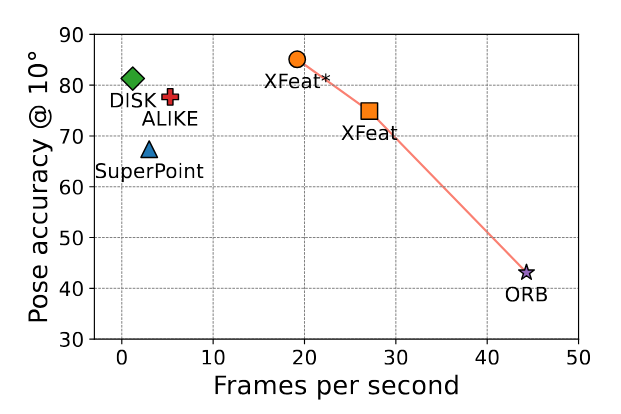
\includegraphics[width=0.8\textwidth]{ressources/xfeat-comparative-graph.png}
    \caption{Comparison of XFeat with other feature matching methods}
    \label{fig:xfeat_architecture}
\end{figure}
\subsection{Datasets}
XFeat utilizes two primary datasets for training and evaluation: the MegaDepth
dataset and a COCO\_20k subset of the COCO2017 dataset. MegaDepth is widely
used in the computer vision community for structure-from-motion and depth
estimation tasks, and XFeat's handling of this dataset is adapted from the
LoFTR official code. The COCO\_20k subset consists of 20,000 images selected
from the full COCO2017 train set, with images chosen based on resolution; this
subset is provided for convenience, but users must adhere to the COCO terms of
use. XFeat's training setup, as described in the accompanying CVPR 2024 paper,
leverages these datasets to achieve robust and efficient keypoint detection and
description, enabling both sparse and semi-dense image matching suitable for
real-world, resource-constrained applications. The datasets provide diverse
scenes and challenges, ensuring that XFeat generalizes well to various
environments, and supporting its goal of real-time, accurate local feature
extraction on standard hardware.
\section{Experimental Design}
\subsection{Data Collection and Preprocessing}
\subsubsection{Icons and Templates}
The data collection process involves handpicking a wide range of game icons and
UI templates that would represent the diversity of visual elements encountered
in gaming environments, while avoiding any flat or smooth icon; as these would
not provide sufficient texture for feature matching.

\begin{figure}[H]
    \centering
    
\includegraphics[width=0.2\textwidth]{ressources/iconexample1.png} \hfill
    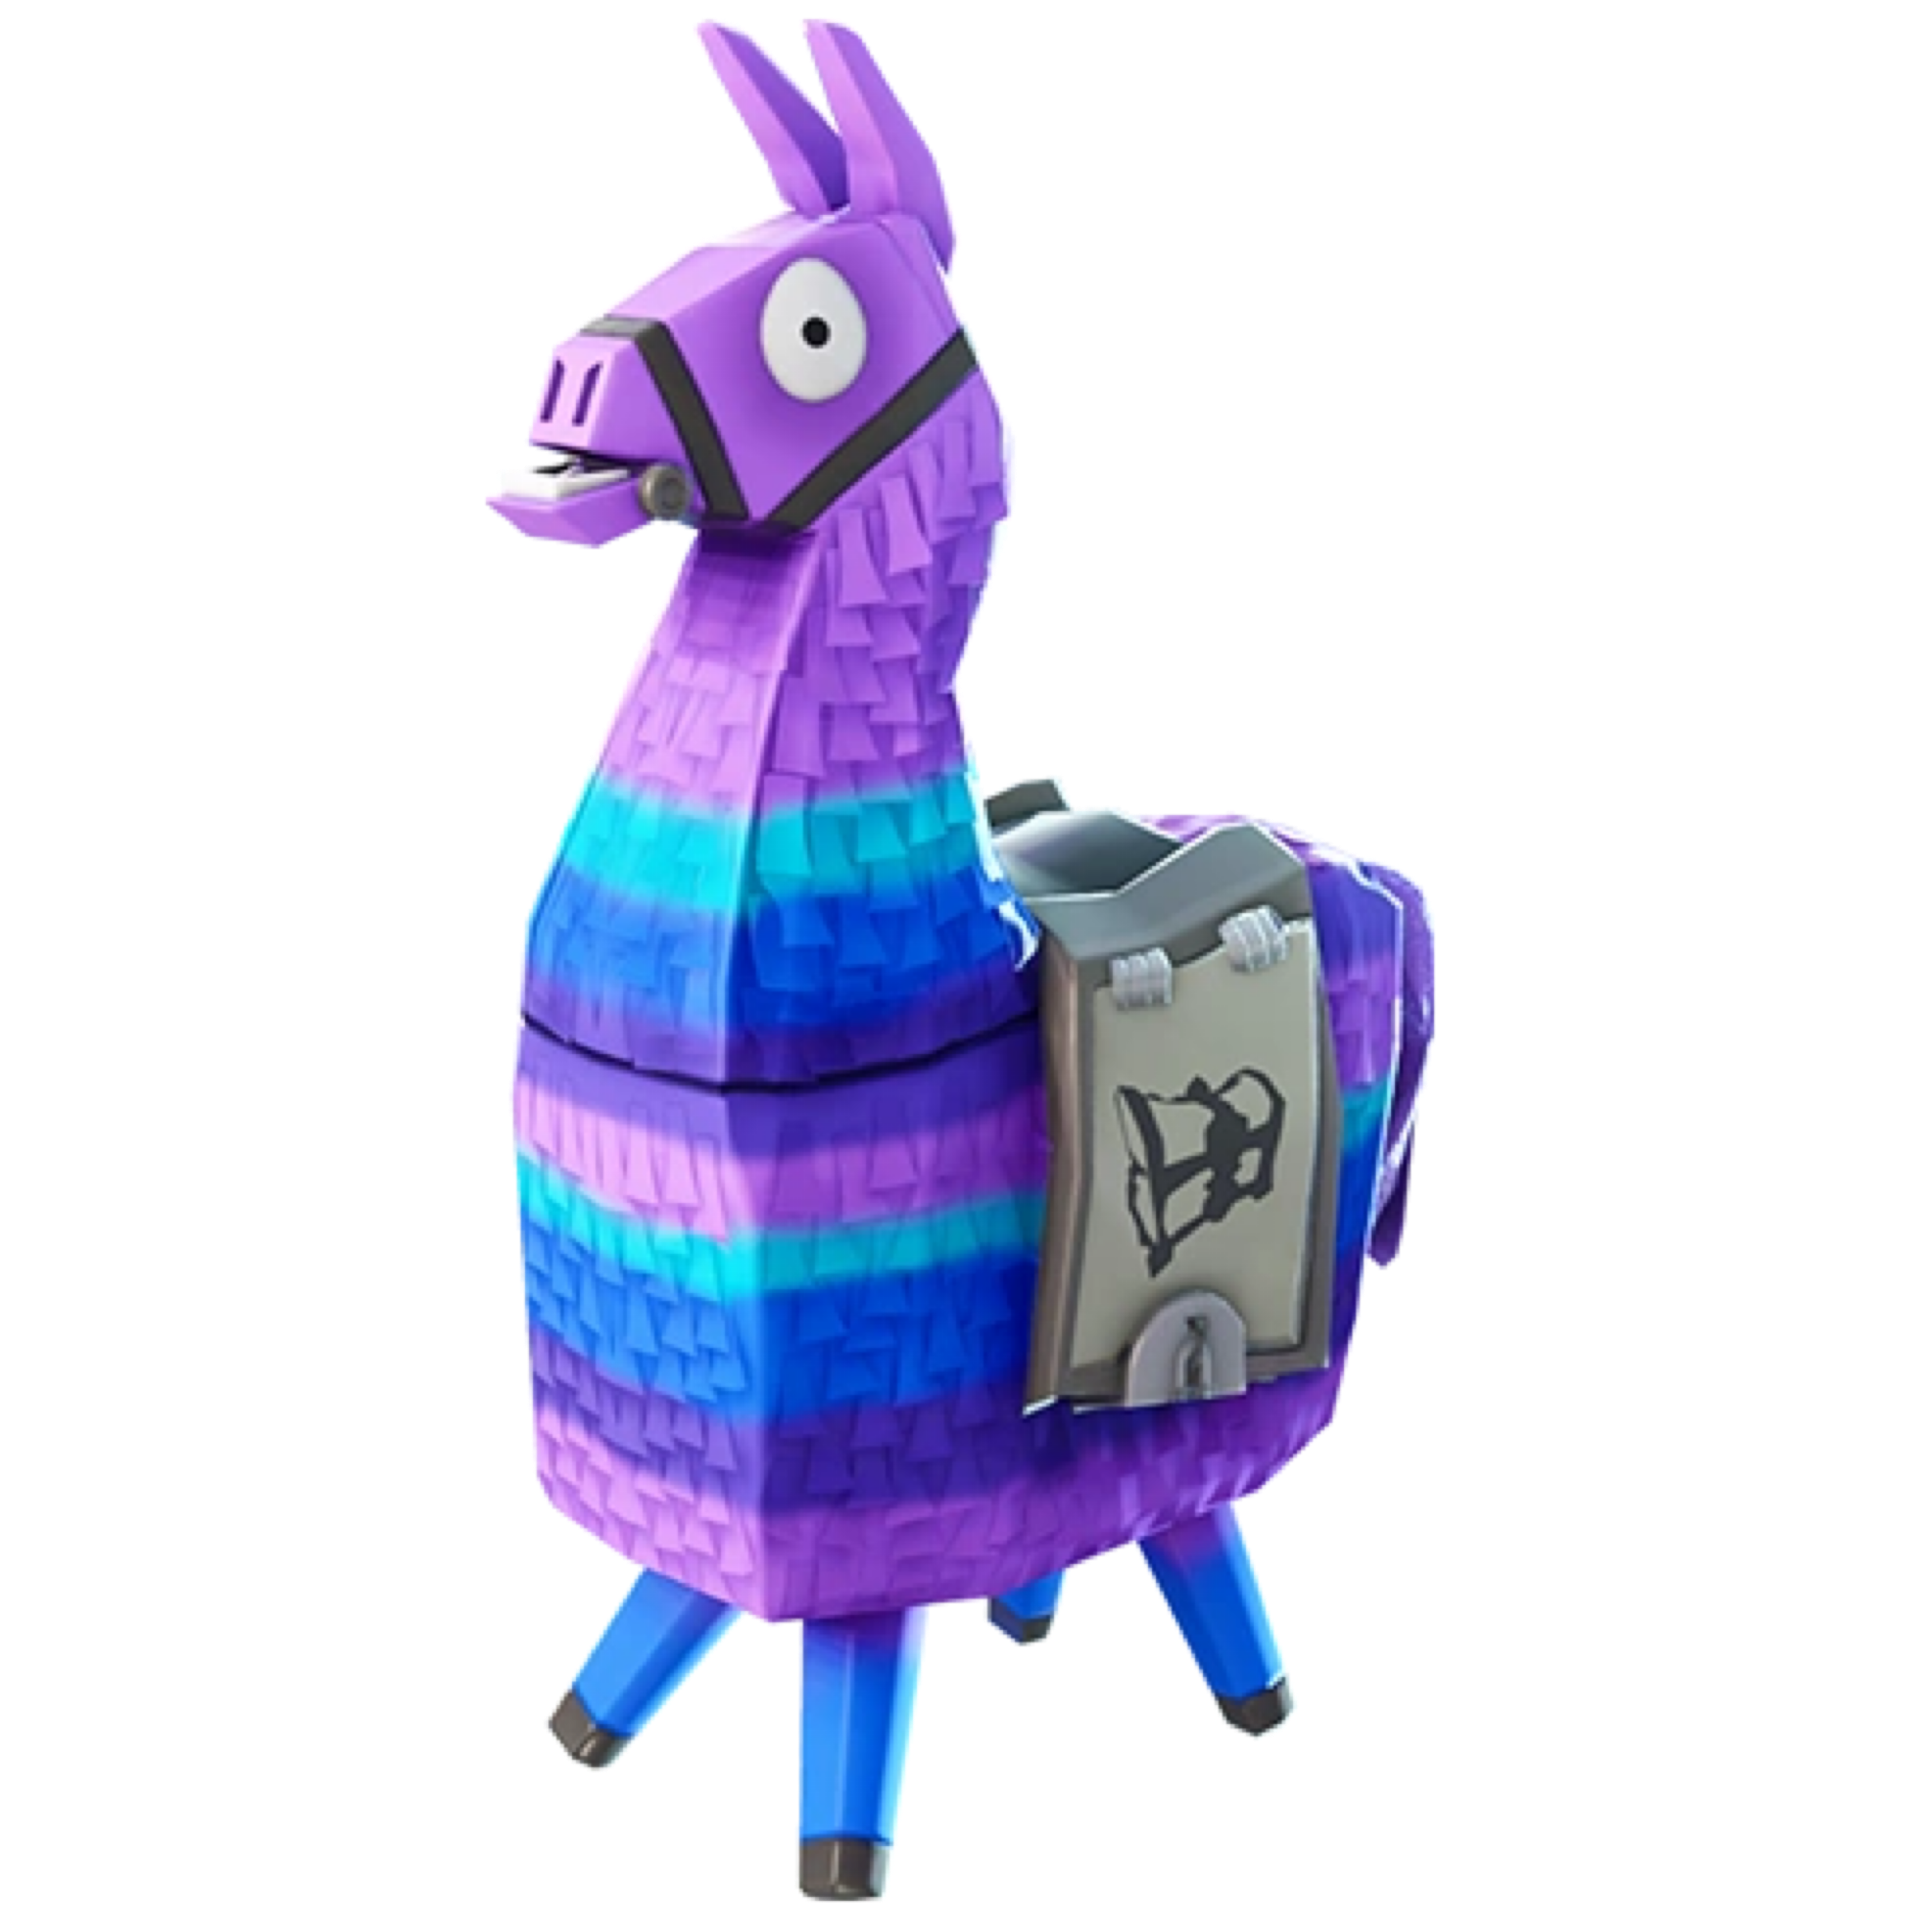
\includegraphics[width=0.2\textwidth]{ressources/iconexample2.png} \hfill
    
\includegraphics[width=0.2\textwidth]{ressources/iconexample3.png} \hfill
    
\includegraphics[width=0.2\textwidth]{ressources/iconexample4.png} \hfill
    \caption{Example of gaming elements used in dataset creation}
    \label{fig:icons}
\end{figure}

\begin{figure}[H]
    \centering
    
\includegraphics[width=0.2\textwidth]{ressources/bad_icon1.png} \hfill
    
\includegraphics[width=0.2\textwidth]{ressources/bad_icon2.png} \hfill
    
\includegraphics[width=0.2\textwidth]{ressources/bad_icon3.png} \hfill
    
\includegraphics[width=0.2\textwidth]{ressources/bad_icon4.png} \hfill
    \caption{Example of gaming elements avoided in dataset creation}
    \label{fig:bad_icons}
\end{figure}
\subsubsection{Footage Collection}
To complete a realistic gaming footage scenario, we have picked random footage
from various TwitchTV streams, focusing on gameplay that prominently features
the UI elements and random backgrounds that could be encountered in real-world
gaming sessions. The footage is then processed to extract frames at a certain
rate, ensuring that the dataset captures dynamic interactions with the UI
elements. Each frame is annotated with the corresponding icons and UI elements
present, allowing for precise evaluation of feature matching performance.

\begin{figure}[H]
    \centering
    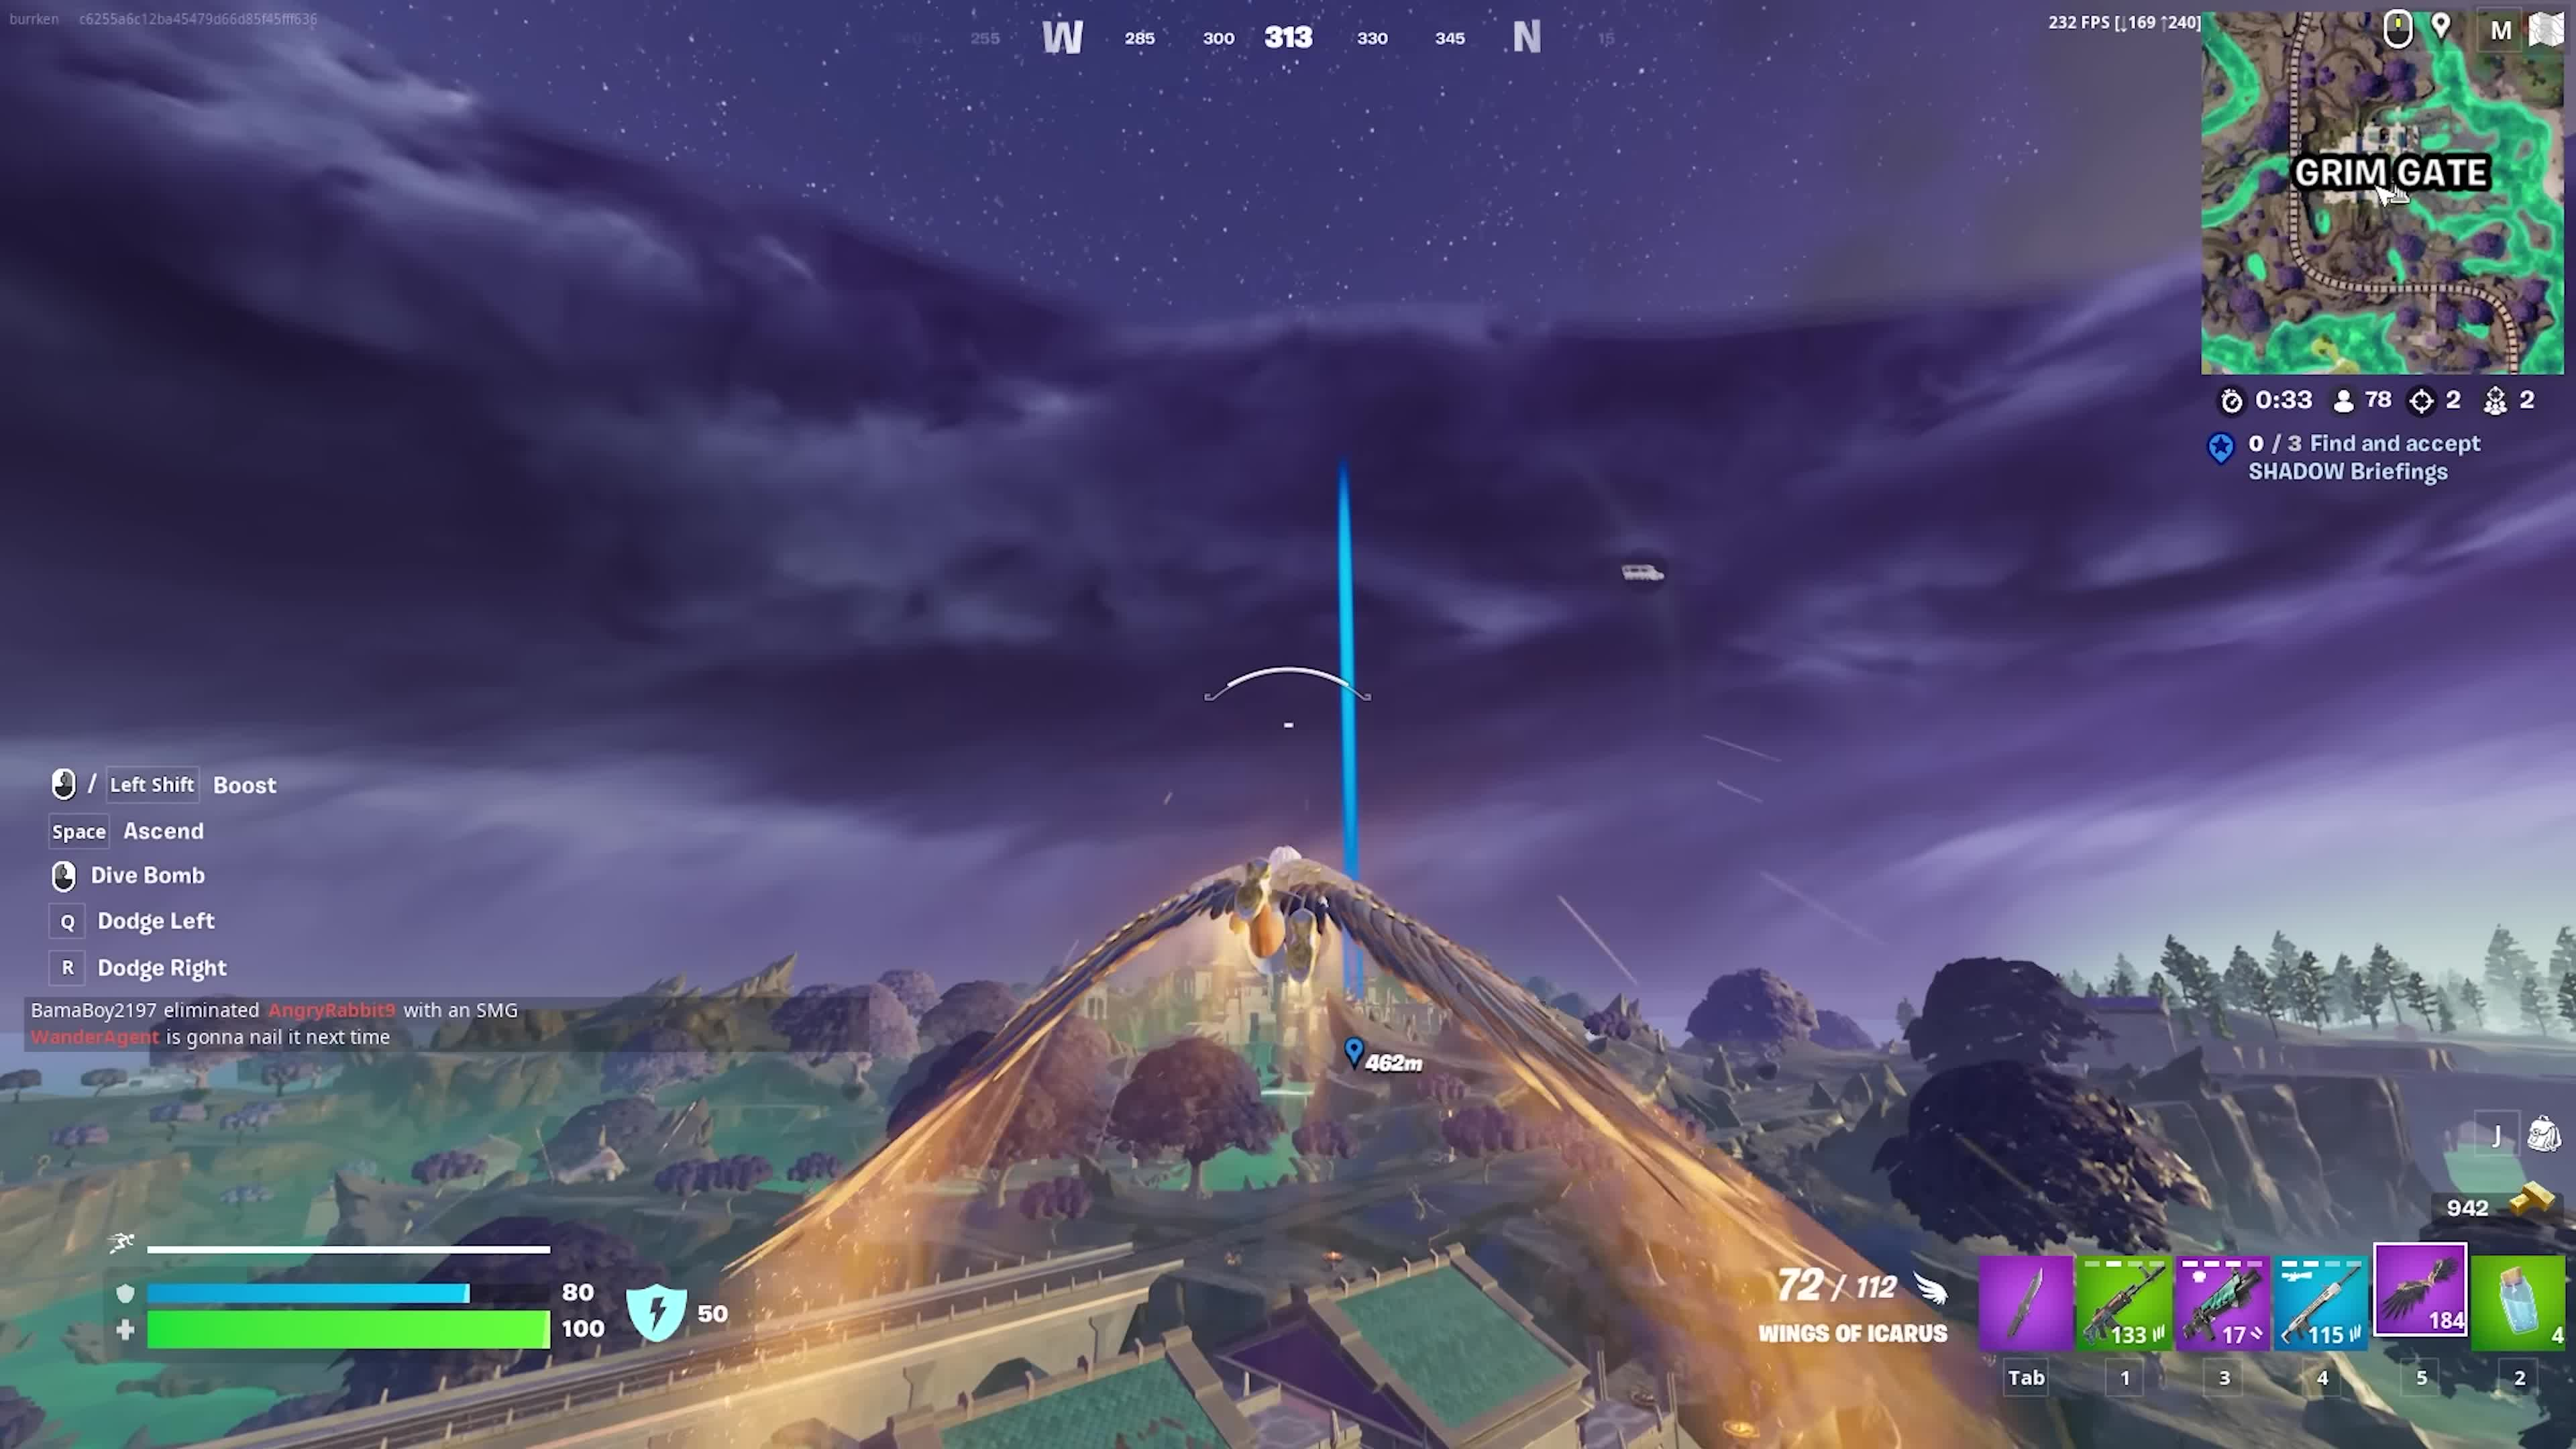
\includegraphics[width=0.8\textwidth]{ressources/bg_example.jpg}
    \caption{Example of backgrounds used in dataset creation}
    \label{fig:background_example}
\end{figure}

This will ensure that the dataset is representative of the actual gaming
environments and provides a solid foundation for training and evaluating the
feature matching.
\subsection{Design of Teacher-Student Framework}
The teacher-student framework is designed to leverage the strengths of both
handcrafted feature matching methods and neural network-based approaches. For
this, we have selected two strong candidates: ALIKE, originally picked by the
authors, and a sophisticated SIFT variant, currently in use at SteelSeries.
Both methods have been used to extract keypoints and match them across our data
samples.
\subsection{SIFT Implementation}
The current solution implemented at SteelSeries leverages a sophisticated SIFT
implementation that enhances the traditional SIFT algorithm for our specific
use case. The implementation goes as follows:

We employ a carefully tuned Scale-Invariant Feature Transform (SIFT) configuration to maximise the number of stable, repeatable keypoints in varied imaging conditions. The detector is initialised with the following parameters:

\begin{itemize}
    \item \textbf{$nOctaveLayers = 4$}: controls the number of scale-space intervals per octave. Increasing this value produces more keypoints across finer scale increments, improving detection in textured or low-detail regions at the cost of additional computation.
    \item \textbf{$contrastThreshold = 0.02$}: sets the minimum contrast required for a candidate keypoint to be retained. Lowering this threshold allows the detector to preserve low-contrast features that may still be distinctive, particularly in low-texture or dim areas, but also increases sensitivity to noise.
    \item \textbf{$edgeThreshold = 5$}: filters out keypoints lying on edges by evaluating the ratio of principal curvatures in the Difference-of-Gaussians response. Lower values are stricter, rejecting more elongated edge responses; our choice balances the removal of unstable edge points with the retention of useful linear features.
    \item \textbf{$\sigma = 1.8$}: specifies the Gaussian smoothing applied at the initial scale of each octave. Larger values increase robustness to noise and small perturbations but can blur fine details; $\sigma = 1.8$ offers a compromise between stability and spatial precision.
\end{itemize}

After detecting keypoints in both the reference and target images, descriptors are computed and normalised by dividing each vector by the sum of its elements. This amplitude normalisation mitigates the effect of overall descriptor magnitude differences, focusing the comparison on relative component values.

Candidate correspondences are generated using a FLANN-based approximate nearest-neighbour search with a KDTree index. For each reference descriptor, the two nearest neighbours in the target descriptor set are retrieved. Match filtering follows a two-pronged strategy:
\begin{enumerate}
    \item \textbf{Relative criterion}: Lowe’s ratio test is applied, retaining matches where the closest neighbour’s distance is less than $0.7$ times that of the second-closest neighbour. This rejects ambiguous matches where multiple candidates are similarly close in descriptor space.
    \item \textbf{Absolute criterion}: Any match with a nearest neighbour distance below $0.09$ is also accepted, even if the ratio test is not satisfied, ensuring that exceptionally strong correspondences are preserved.
\end{enumerate}

The filtered matches are recorded as index pairs into the respective keypoint arrays. This combination of tuned detector parameters, descriptor normalisation, and dual match filtering yields a set of correspondences that is both distinctive and resilient to background clutter and illumination changes.
 \section{Evaluation metrics} %TODO

% ------------------------------------------------------------
\chapter{Implementation, Result, and Analysis}
\section{Overview of the approach}
Before training, we have reviewed what the chosen network requires as input.
Since we are training using synthetic dataset that would imitate our target
scenarios, we focused on generating diverse and representative samples.
\section{Dataset Preparation \& Preprocessing}
The network expects:
\begin{itemize}
    \item \textbf{Two images:} the reference image, and the target image. Stored as numpy arrays.
    \item \textbf{Two sets of keypoints:}
          \begin{itemize}
              \item \textbf{Reference keypoints:} An array of keypoint coordinates found in the reference
                    image. It has a shape of $(N, 2)$, where N is the number of keypoints, and the coordinates are (x, y).
              \item \textbf{Target keypoints:} An array of keypoint coordinates found in the target image that correspond to the reference keypoints. It has the same shape $(N, 2)$.
          \end{itemize}
    \item \textbf{Matches:} An array of shape $(N, 2)$ that stores the indices of the matching keypoints. For example, $[i, j]$ means that the i-th keypoint in the reference keypoints matches the j-th keypoint in the target keypoints.
    \item \textbf{Homography Matrix: } A 3 by 3 matrix that relates the reference icon to the target one. It is used to transform points from the reference to the target image, and vice versa.
    \item \textbf{Two binary masks:} Binary masks of the target image that indicates the region where the pixel exists. This is useful to separate the foreground from the background.
\end{itemize}
These elements would be stored as a zipped numpy file (.npz) to be later accessed during training and evaluation, and stored in a folder structure that mirrors the dataset organization.
\subsection{Data Synthesis}
\subsubsection{General Approach}
To create a diverse and representative dataset, we employed data synthesis
techniques that will allow us to experiment with various scenarios. Our general
idea consists of cropping a region of interest from the selected gaming frames,
this will help us simulate different viewpoints where the targeted 2D template
may appear.
\begin{figure}[H]
    \centering
    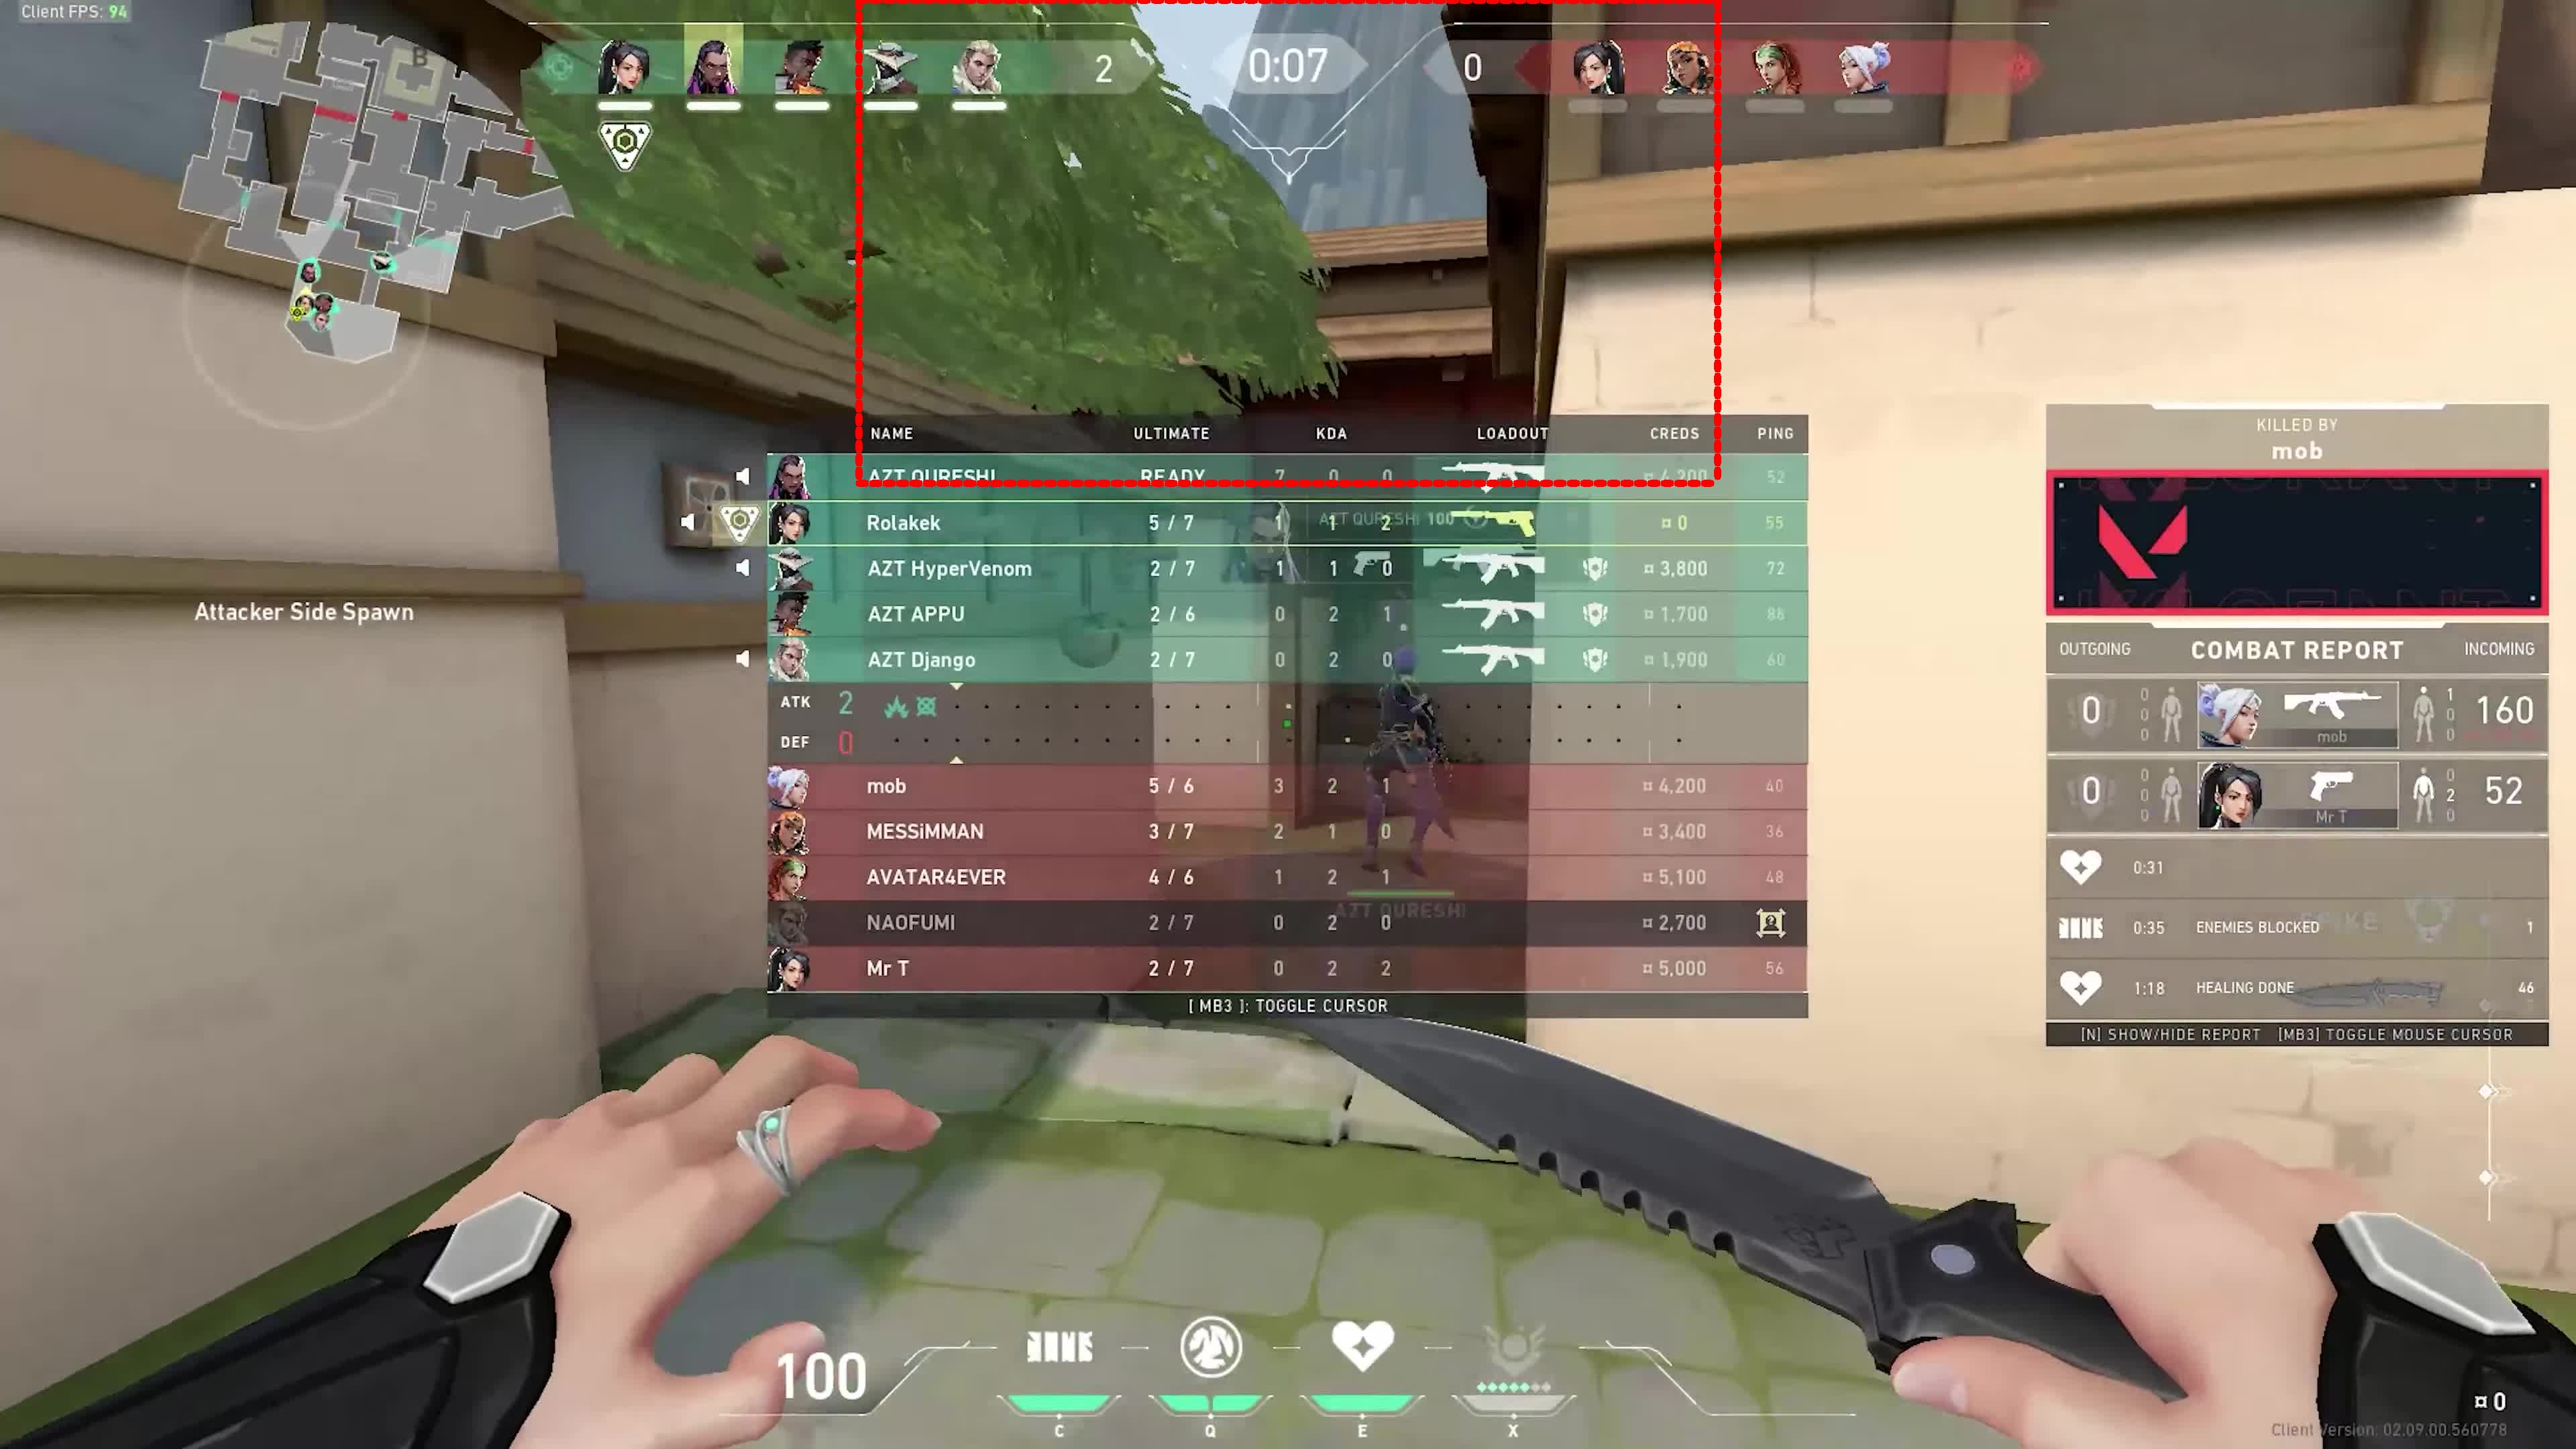
\includegraphics[width=\textwidth]{ressources/roi.jpg}
    \caption{Example of a cropped region of interest from a gaming frame.}
    \label{fig:roi_example}
\end{figure}
This newly selected area will serve as our background for the rest of the synthesis process. Then, we select an icon from our set of templates, which will be our target during training. We overlay our icon onto the background at the center, and we ensure that the icon is fully contained within the background region by downscaling it slightly and continuously till it fits perfectly.
\begin{figure}[H]
    \centering
    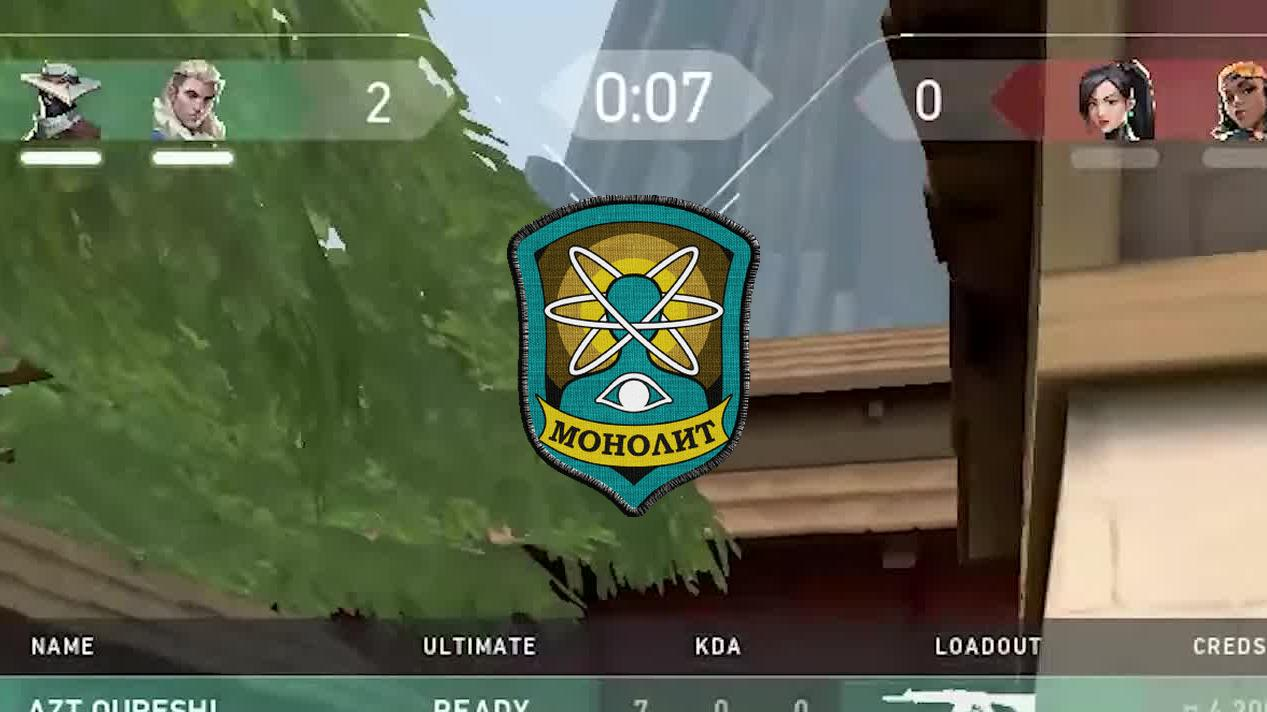
\includegraphics[width=0.9\textwidth]{ressources/image1.jpg}
    \caption{Example of the icon overlaid on the background.}
    \label{fig:overlay_example}
\end{figure}
While this describes our general design principle for synthetic data generation, the process was refined over several iterations to address specific challenges such as background complexity, icon transformations, and the robustness of extracted keypoints.
\begin{comment}
\begin{itemize}
    \item Scaling: We randomly scale the icon by a factor between 1.0 and 3.0
    \item Rotation: We randomly rotate the icon by an angle between -30 and 30 degrees.
    \item Translation: We randomly translate the icon by a few pixels in both x and y
          directions, while insuring that the icon remains within the bounds of the
          background.
    \item Color Jittering: We apply random changes to the brightness, contrast,
          saturation, and hue of the icon to create variations in appearance.
    \item Gaussian Noise: We add random Gaussian noise to the icon to simulate real-world
          noise.
\end{itemize}
\end{comment}

\section{Training Procedure \& Experimental Setup}
Our chosen approach consists of training the network on synthetic data using a
teacher-student framework. In the early stages, we kept the same teacher model
used by XFeat\cite{xfeat2023}. ALIKE, was used as a third party teacher tool to
extract ground truth keypoints from our training images.
\begin{figure}[H]
    \centering
    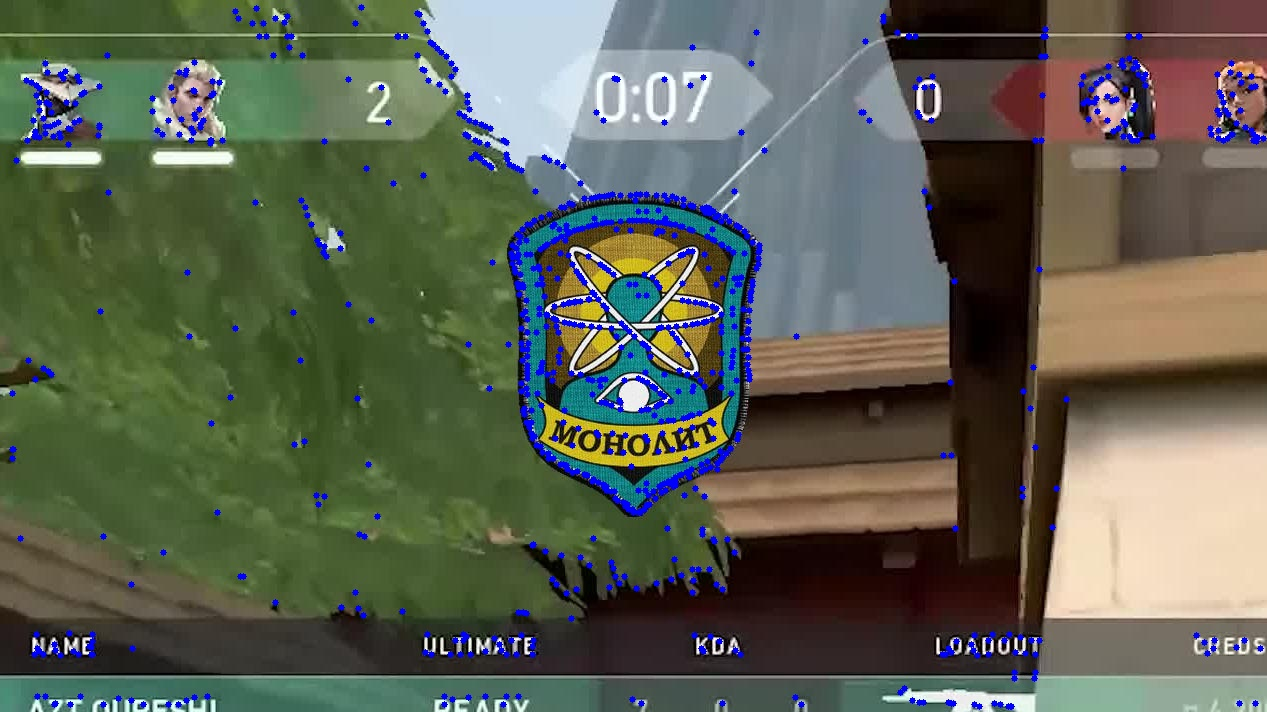
\includegraphics[width=0.8\textwidth]{ressources/image1_keypoints.jpg}
    \caption{Overview of extraction process.}
    \label{fig:teacher_student}
\end{figure}
We then generate a binary mask showing the presence of the icon within the background.
\begin{figure}[H]
    \centering
    
\includegraphics[width=0.8\textwidth]{ressources/mask_1.png}
    \caption{Example of the binary mask generated for the icon.}
    \label{fig:binary_mask}
\end{figure}
This mask is used to filter out keypoints that do not belong to the icon, ensuring that only relevant features are considered during training. This would teach the model to focus only the keypoints and data existing within the icon region , which is what we want to achieve.
\begin{figure}[H]
    \centering
    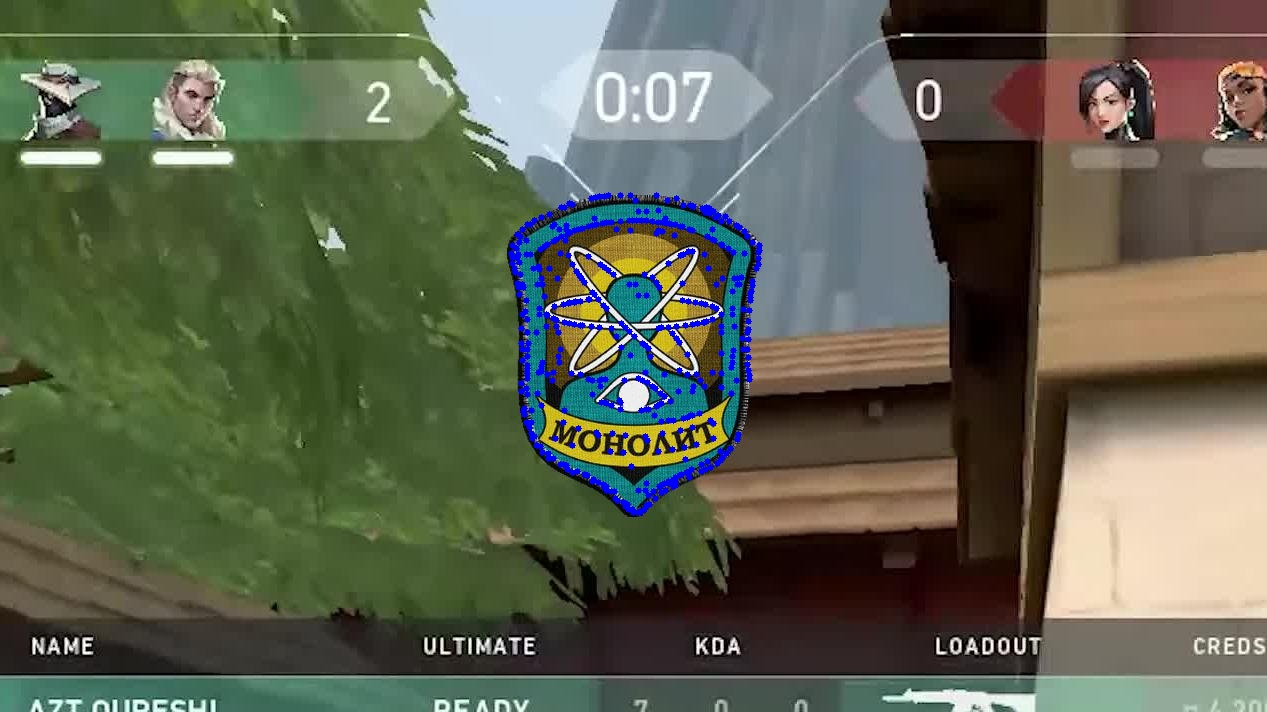
\includegraphics[width=0.8\textwidth]{ressources/image1_keypoints_masked.jpg}
    \caption{Overview of filtering process.}
    \label{fig:teacher_student}
\end{figure}
By repeating this process on both \textbf{reference} and \textbf{target} images, we get a pair of keypoint arrays ready to match using ALIKE's matching algorithm to finally get our training data samples.

\begin{figure}[H]
    \centering
    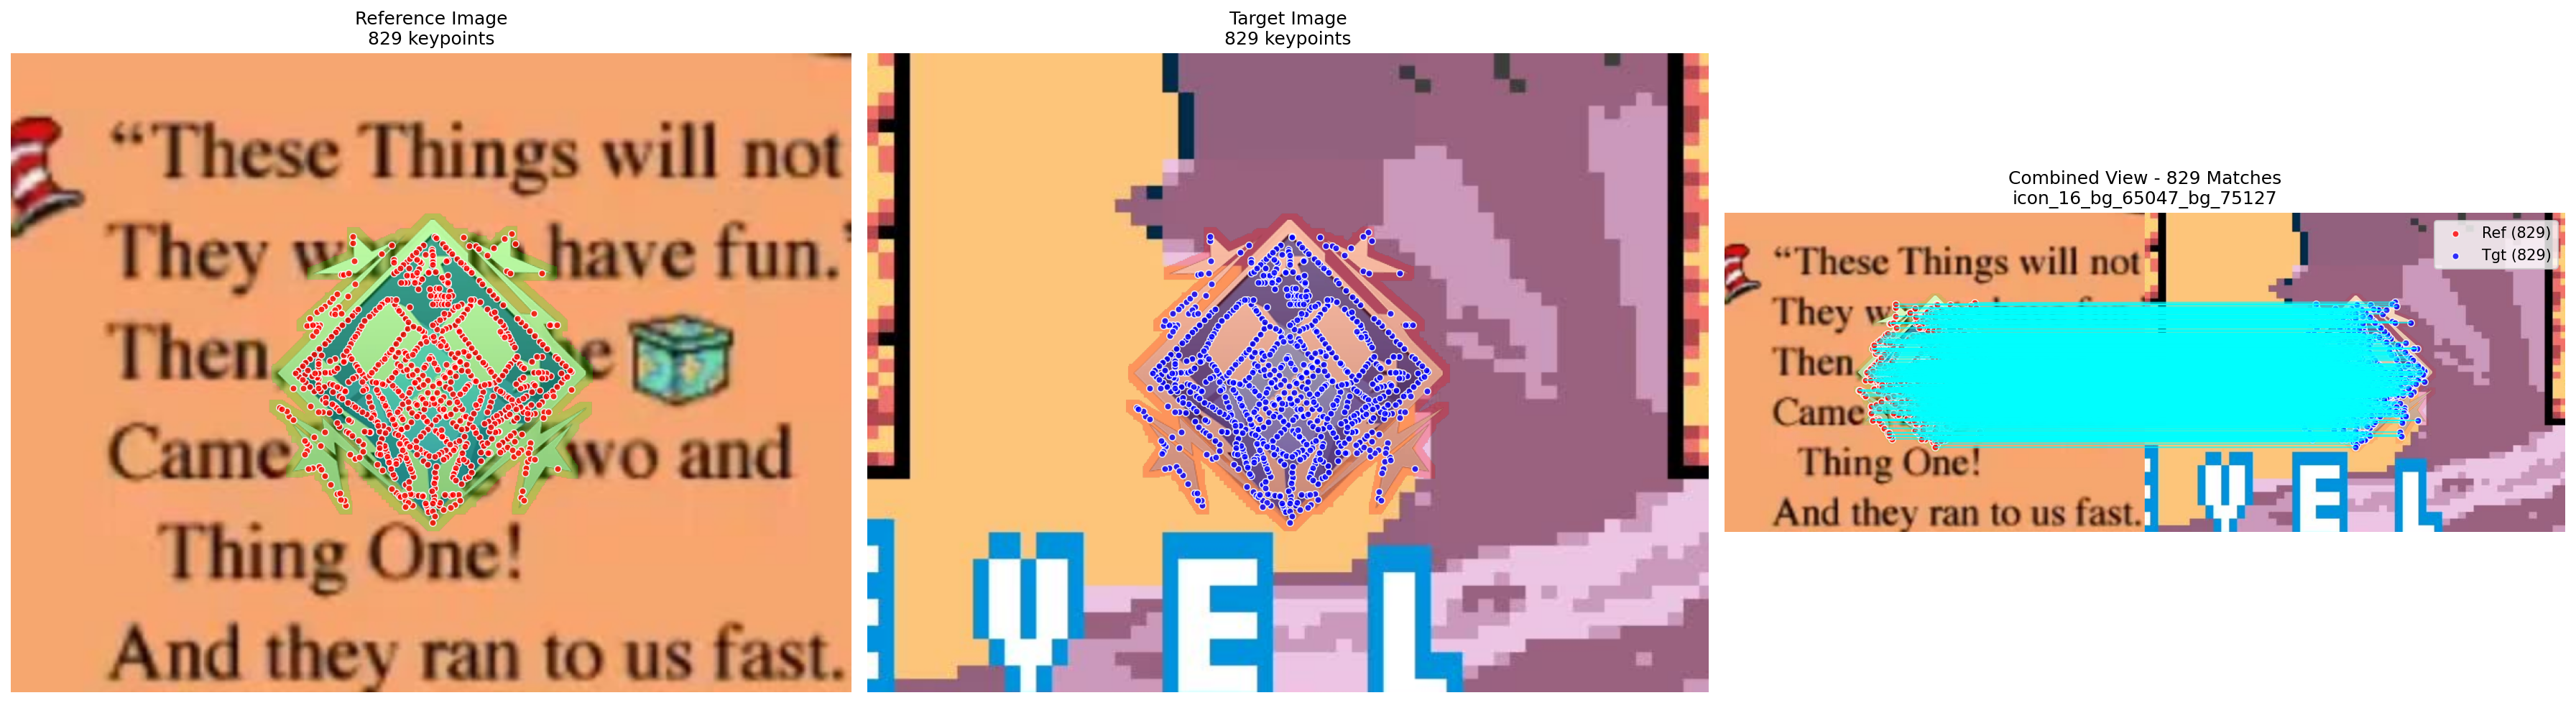
\includegraphics[width=\textwidth]{ressources/example_data1.png}
    \caption{Example of the synthesis process, showing the background and the overlaid icon as well as the detected keypoints and masks.}
    \label{fig:synthesis_example1}
\end{figure}
At a first time we trained the model following the default parameters:
\begin{itemize}
    \item Learning rate: 0.001
    \item Batch size: 10
    \item Number of iterations: 160k
\end{itemize}
This has led us to under average results, prompting further investigation into hyperparameter tuning and data formulation.
\subsection{Results}
The metrics obtained from our initial training runs indicate that while the
model is capable of learning the basic features of the icons, it struggles with
more complex backgrounds and variations in icon appearance.
\begin{figure}[H]
    \centering
    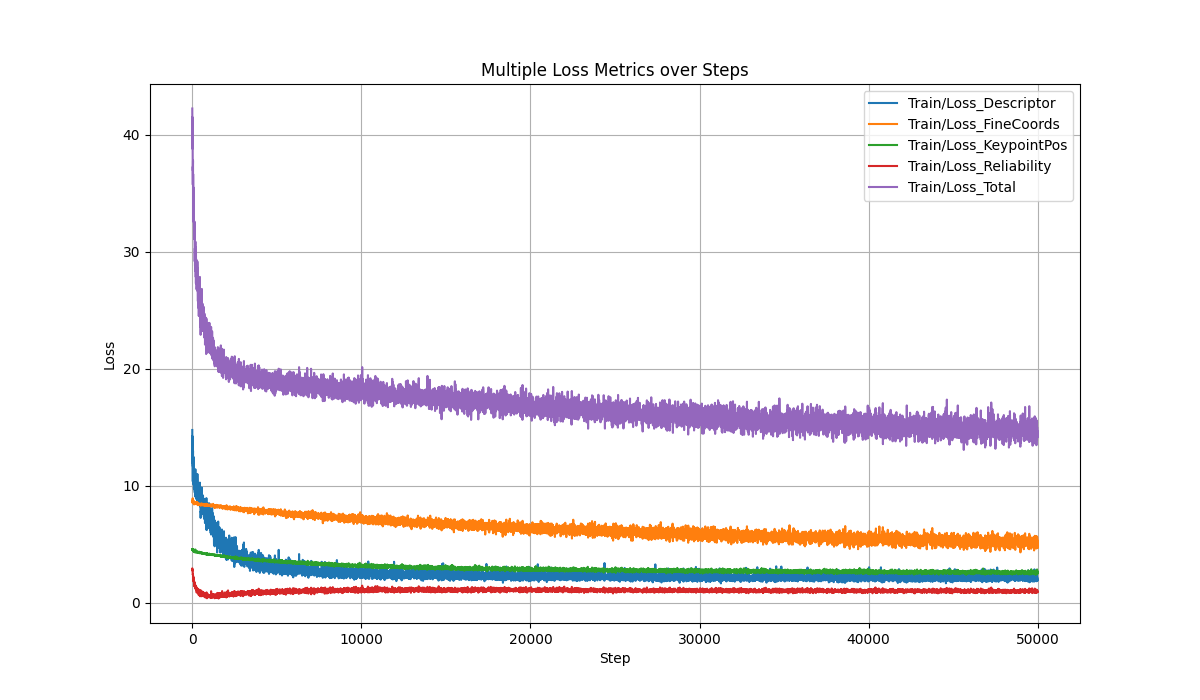
\includegraphics[width=\textwidth]{ressources/loss_1.png}
    \caption{Loss curves for initial training runs.}
    \label{fig:loss_curves_1}
\end{figure}
\begin{figure}[H]
    \centering
    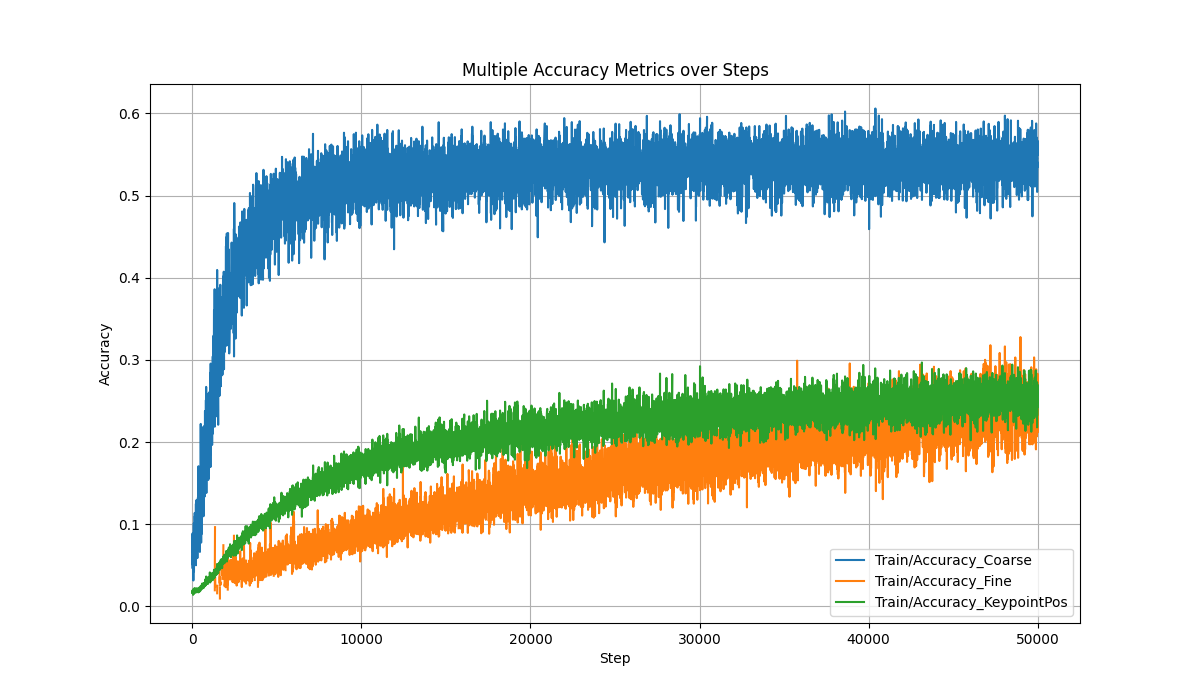
\includegraphics[width=\textwidth]{ressources/acc_1.png}
    \caption{Accuracy curves for initial training runs.}
    \label{fig:acc_curves_1}
\end{figure}
\subsubsection{Accuracy Metrics}
\begin{itemize}
    \item \textcolor{blue}{\textbf{Coarse Accuracy: }}Rapid increase in the first ~5k steps, reaching ~55\%-60\%. Then it plateaus with small oscillations.
    \item \textcolor{darkgreen}{\textbf{Keypoint Position Accuracy: }}Steady growth until ~20k steps, then saturates around ~25\%-27\%.
    \item \textcolor{myorange}{\textbf{Fine Matching Accuracy: }}Slow but consistent improvement, reaching ~20\%-22\% by step 50k, with more variance in later steps.
\end{itemize}
We can interpret this as follows:
\begin{itemize}
    \item The model learns coarse correspondences very quickly and maintains that
          performance, suggesting early layers or coarse matching blocks converge fast.
    \item Fine matching is the slowest to improve, likely because it depends on the
          coarse stage being strong first, and needs more subtle feature learning.
    \item Keypoint position accuracy plateaus mid-training, meaning spatial localization
          stops improving after ~20k steps.
\end{itemize}
\subsubsection{Loss Metrics}
\begin{itemize}
    \item \textcolor{blue}{\textbf{Descriptor Loss: }}Sharp drop in the first $\sim$5k steps, then remains low and stable (around 1--2).
    \item \textcolor{myorange}{\textbf{Fine Coordinates Loss: }}Slow but steady decrease across the 50k steps, still trending down by the end of training.
    \item \textcolor{darkgreen}{\textbf{Keypoint Position Loss: }}Drops quickly in early training and stabilizes, mirroring the accuracy plateau.
    \item \textcolor{red}{\textbf{Reliability Loss: }}Low from the start with minimal change, indicating stable confidence estimation.
    \item \textcolor{purple}{\textbf{Total Loss: }}Large drop in the first $\sim$5k steps, followed by a slower but continuous decline until the end.
\end{itemize}

We can interpret this as follows:
\begin{itemize}
    \item Most of the learning happens in the first 5k--10k steps, especially for
          descriptors and keypoint positioning.
    \item Fine coordinate refinement remains the main bottleneck, as its loss is still
          higher and accuracy is still improving, suggesting more training could help.
    \item Reliability loss stability shows that confidence estimation remains consistent
          throughout training.
\end{itemize}

\subsubsection{Confusion matrix}
\begin{figure}[H]
    \centering
    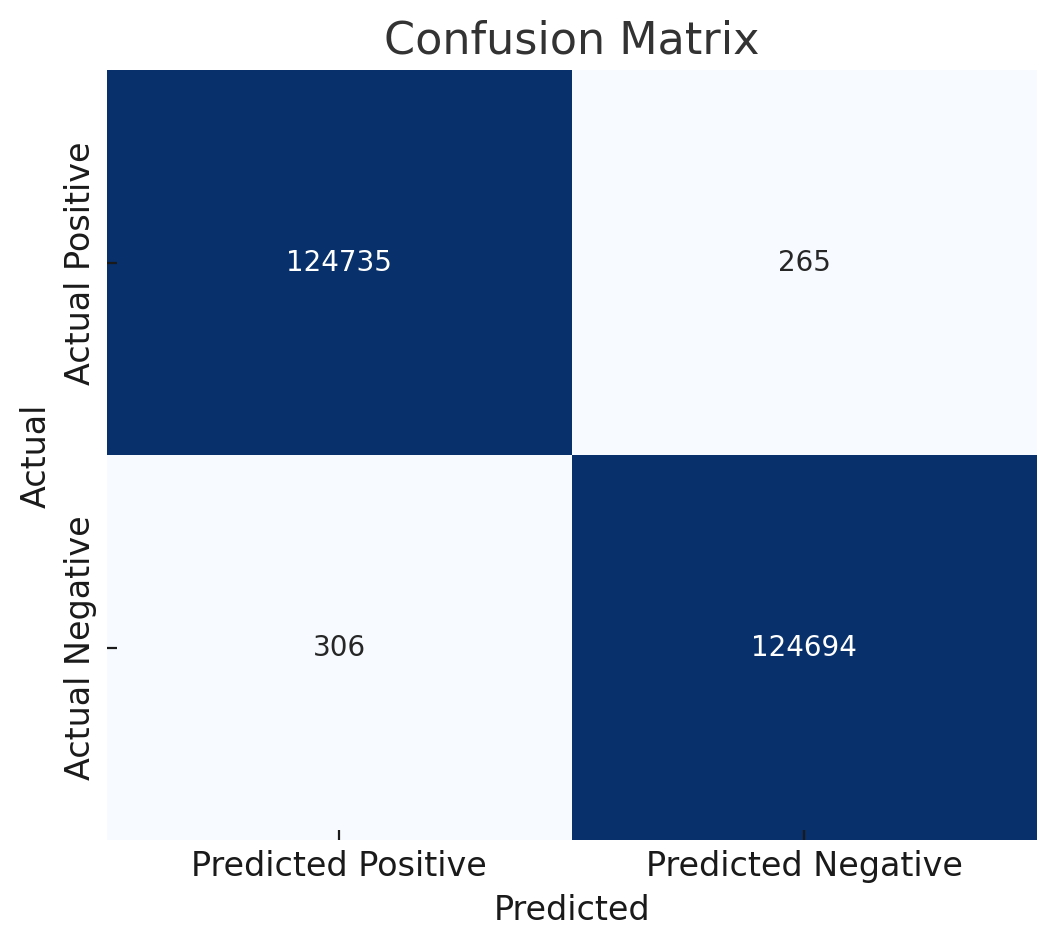
\includegraphics[width=0.7\textwidth]{ressources/confusion_matrix_1.png}
    \caption{Confusion matrix for initial training runs.}
    \label{fig:confusion_matrix_1}
\end{figure}
The confusion matrix shows the following values:
\begin{itemize}
    \item \textbf{True Positives (TP):} 124,735 cases where positive samples were correctly classified.
    \item \textbf{False Negatives (FN):} 265 cases where positive samples were incorrectly classified as negative.
    \item \textbf{False Positives (FP):} 306 cases where negative samples were incorrectly classified as positive.
    \item \textbf{True Negatives (TN):} 124,694 cases where negative samples were correctly classified.
\end{itemize}

From these values, we can compute:
\begin{itemize}
    \item \textbf{Accuracy:} $\frac{TP + TN}{TP + TN + FP + FN} \approx 99.77\%$
    \item \textbf{Precision:} $\frac{TP}{TP + FP} \approx 99.76\%$
    \item \textbf{Recall:} $\frac{TP}{TP + FN} \approx 99.79\%$
    \item \textbf{F1-Score:} $\approx 99.78\%$
\end{itemize}

These results indicate that the model performs extremely well, with both
precision and recall above 99.7\%, suggesting minimal misclassification in both
classes, but not enough, as False positives are extremely important in our
case, as they would lead to false matches, and ultimately impact the user
experience negatively.
\subsubsection{Overall Assessment}
The training shows strong performance in terms of fast convergence on coarse
matching and descriptor learning, with stable behavior and no signs of
divergence. However, fine matching accuracy remains low compared to coarse
accuracy, and keypoint accuracy saturates early, indicating possible
underfitting in fine localization. \textbf{To address these issues, several
    strategies can be considered: extending the training or applying fine-tuning
    with a smaller learning rate to further improve fine accuracy, reweighting the
    losses to give more emphasis to the FineCoords component once the coarse stage
    has converged, and applying data augmentation techniques that highlight
    sub-pixel differences to strengthen fine matching capabilities. Additionally, a
    curriculum learning approach could be adopted, starting with simpler examples
    before progressively increasing difficulty for the fine stage. }

\section{Iterative Refinement}
During experimentation, we implemented and evaluated three alternative
synthesis pipelines derived from our general concept:
\begin{enumerate}
    \item \textbf{NAFM A – Static Background-Icon, Transformed Keypoints:}
          The background and icons remained unchanged, while the keypoints were transformed using the homography matrix generated during the synthesis process. This matrix was applied to map the keypoints from the reference image to the target image, rather than re-extracting them from both images using the teacher model.
    \item \textbf{NAFM B – Cropped Background/Dynamic Icon-Transformed Keypoints:}
          The reference image was cropped down to focus on the area of interest, and ignore the background. The target icon was transformed using translation, placing it in a random position within the background.
    \item \textbf{NAFM C – Unfiltered SIFT Features}
          The reference and target images were not changed from the variant B, but the keypoints were extracted and matched using SIFT, without filtering them using the binary mask.
\end{enumerate}
Each variant maintained the core pipeline (ROI selection, overlay, keypoint extraction, matching), but emphasized different aspects of visual variability.
\subsection{Variant A}
In variant A, we focused on maintaining a static background and icon, while
transforming the keypoints obtained from the reference image to the target
image using a homography matrix. This would allow us to generate high quality
matches, as our objective is to find absolute correspondences between the
reference and the query templates. So we thought that using the transformed
keypoints would yield better results than re-extracting them from the target
image.
\subsubsection{Homography-based keypoint transfer}

Let the reference keypoints be $\mathcal{X}=\{ \mathbf{x}_i \}_{i=1}^{N}$ with
$\mathbf{x}_i=(u_i,v_i)^\top$ in pixel coordinates. Write them in homogeneous
form $\tilde{\mathbf{x}}_i=(u_i,v_i,1)^\top$. Let the homography be
$H\in\mathbb{R}^{3\times 3}$.

The mapped keypoints on the target image are
\[
    \tilde{\mathbf{x}}'_i \sim H\,\tilde{\mathbf{x}}_i,
    \qquad
    \mathbf{x}'_i=\Big(\frac{\tilde{u}'_i}{\tilde{w}'_i},\,
    \frac{\tilde{v}'_i}{\tilde{w}'_i}\Big)^\top,
\]
where $\tilde{\mathbf{x}}'_i=(\tilde{u}'_i,\tilde{v}'_i,\tilde{w}'_i)^\top$. In
matrix form for all points:
\[
    \tilde{X}' \sim H \tilde{X}, \quad
    X'=\begin{bmatrix}
        \tilde{X}'_{1,:}/\tilde{X}'_{3,:} \\[2pt]
        \tilde{X}'_{2,:}/\tilde{X}'_{3,:}
    \end{bmatrix}^{\!\top}.
\]

\paragraph{Notes.}
If $\tilde{w}'_i=0$ the point maps to infinity and is discarded.

\begin{figure}[H]
    \centering
    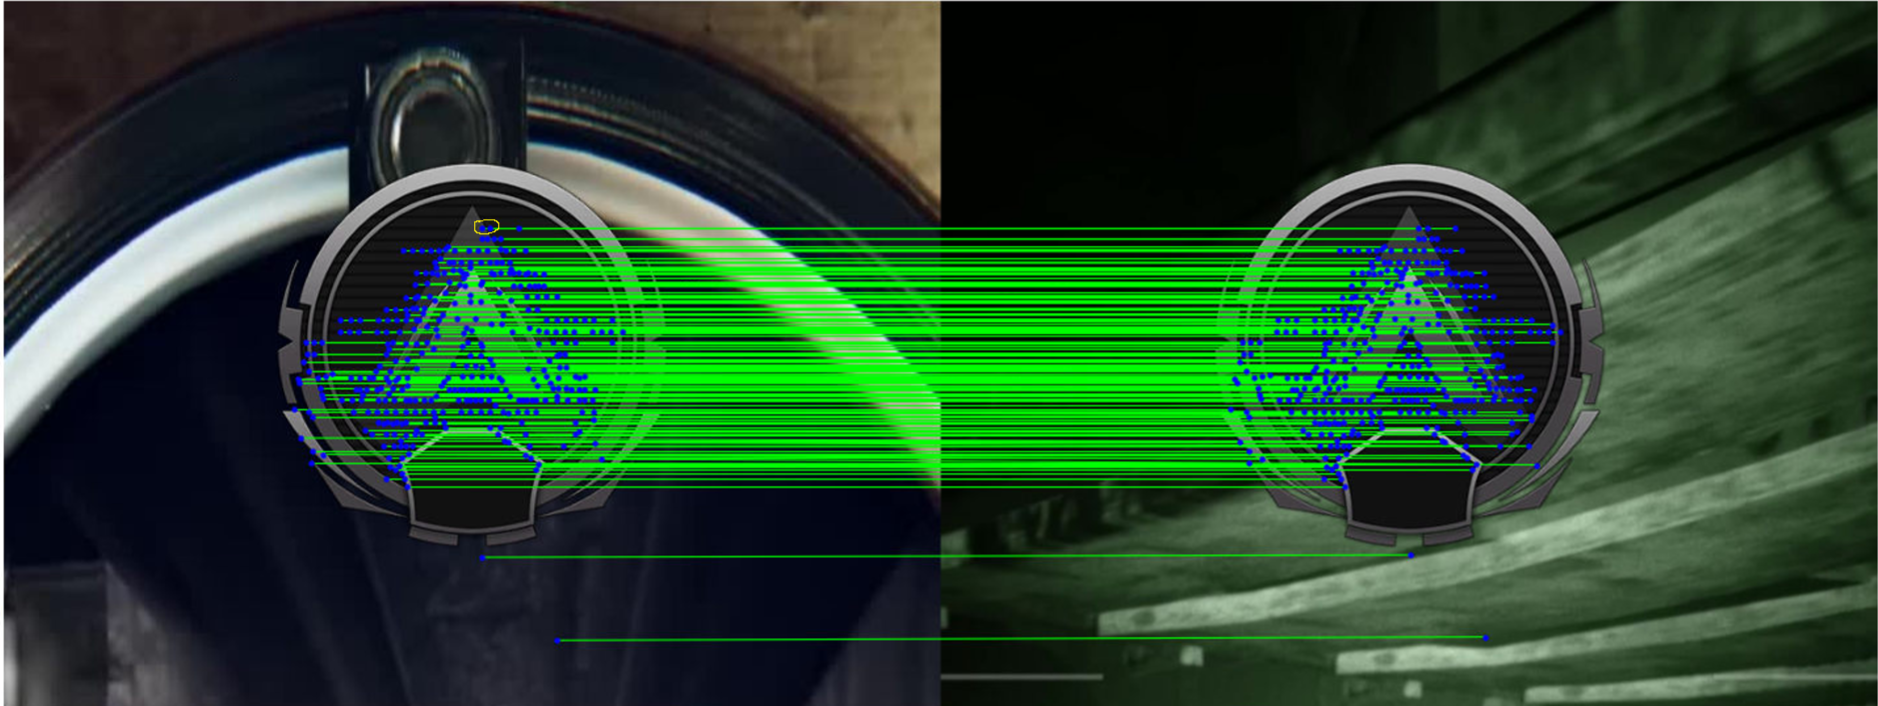
\includegraphics[width=0.6\textwidth]{ressources/image2.png}
    \caption{Example of the synthesis process for variant A}
    \label{fig:variant_a}
\end{figure}

Although this approach seems promising, it relies heavily on the quality of our
data synthesis process, and the homography matrix generation. In practice, we
found that the performance was sensitive to these factors.
\subsubsection{Accuracy metrics}
\begin{figure}[H]
    \centering
    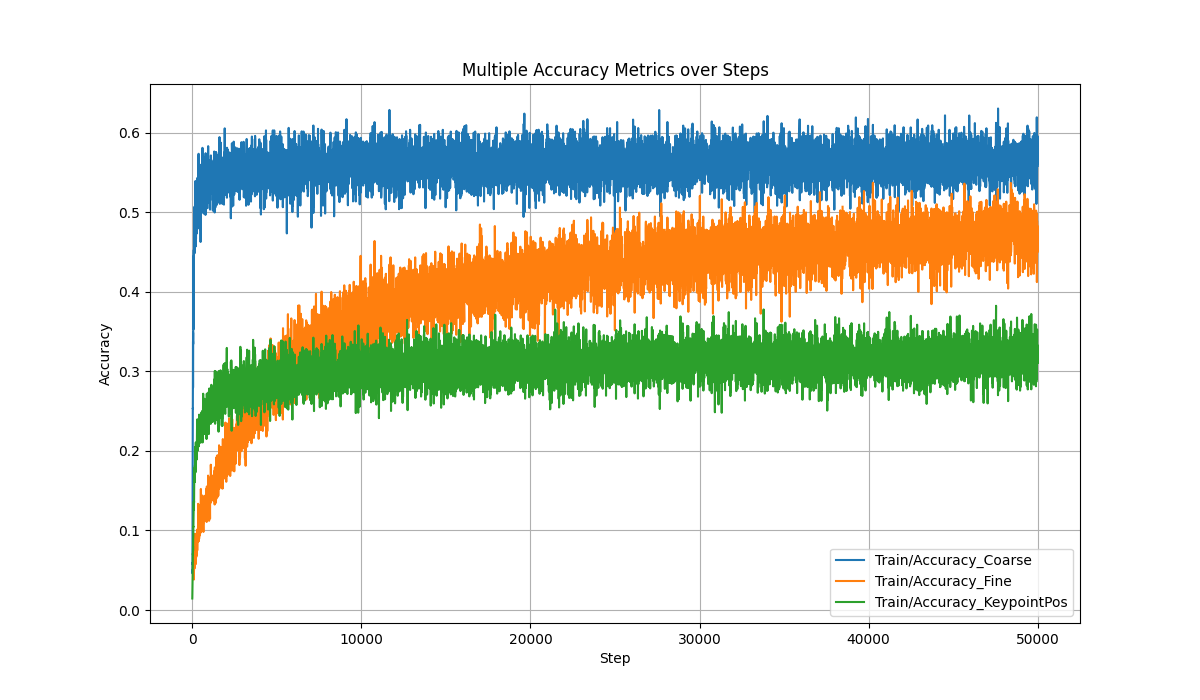
\includegraphics[width=0.7\textwidth]{ressources/acuracy_2.png}
    \caption{Example of the accuracy metrics evaluation}
    \label{fig:accuracy_metrics_2}
\end{figure}
\begin{itemize}
    \item \textcolor{blue}{\textbf{Coarse Accuracy: }}Starts low (~55\%) and quickly stabilizes around 60\%. Stable without large oscillations — suggests the coarse-level model component converged early.
    \item \textcolor{myorange}{\textbf{Fine Accuracy: }}Gradual increase from ~20\% to ~47\% over training — indicates steady improvement in fine-grained matching.
    \item \textcolor{darkgreen}{\textbf{Keypoint Position: }}Rises from ~10\% to ~36\%, slower than coarse accuracy, but still trending upward — likely due to higher difficulty of precise keypoint localization.
\end{itemize}
\subsubsection{Loss metrics}
\begin{figure}[H]
    \centering
    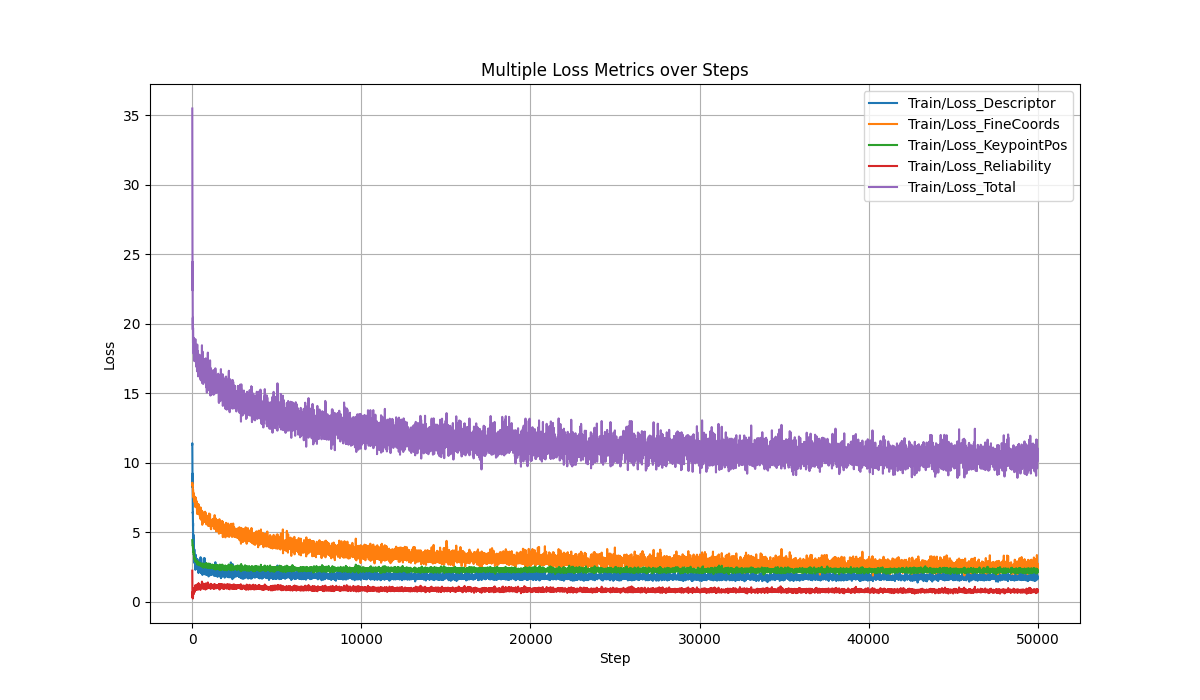
\includegraphics[width=0.7\textwidth]{ressources/multiple_losses_graph_2.png}
    \caption{Example of the loss metrics evaluation}
    \label{fig:loss_metrics_2}
\end{figure}
\begin{itemize}
    \item \textcolor{blue}{\textbf{Descriptor Loss:}} Rapid drop from ~17 to ~1.5 in the first 5k–10k steps, then slow decline — feature descriptors are learning quickly.
    \item \textcolor{myorange}{\textbf{Fine Coords Loss:}} Drops from ~8 to ~2.2, showing better coordinate regression.
    \item \textcolor{darkgreen}{\textbf{Keypoint Position Loss:}} Drops from ~4.5 to ~2.2 — still higher than fine coords, implying room for improvement in keypoint position accuracy.
    \item \textcolor{purple}{\textbf{Reliability Loss:}} Drops from ~2.5 to ~1.0 — confidence estimation is improving.
    \item \textcolor{red}{\textbf{Total Loss:}} Drops sharply from ~45 to ~12–14, then plateaus — convergence reached.
\end{itemize}
\subsubsection{Confusion Matrix}
\begin{figure}[H]
    \centering
    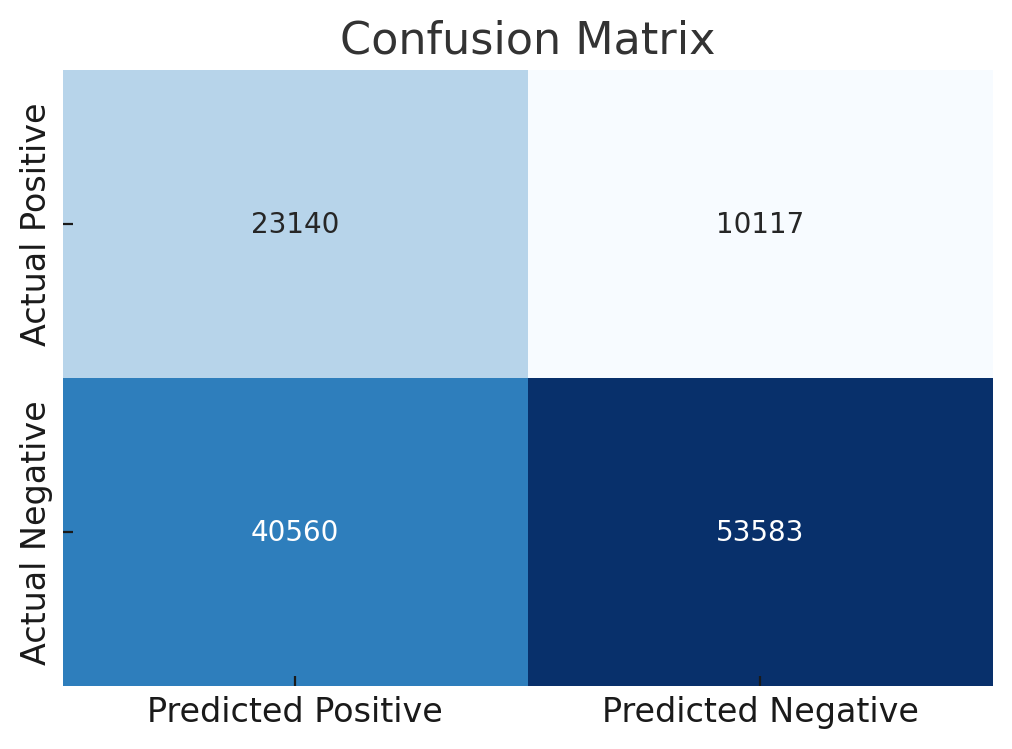
\includegraphics[width=0.6\textwidth]{ressources/confusion_matrix_2.png}
    \caption{Confusion matrix for variant A}
    \label{fig:confusion_matrix_2}
\end{figure}
\begin{itemize}
    \item \textbf{Accuracy :} 0.602
    \item \textbf{Precision :} 0.696
    \item \textbf{Recall :} 0.363
    \item \textbf{F1 Score :} 0.477
\end{itemize}
\subsubsection{Interpretation}
The results show that while the model can differentiate between various
features and capture some general patterns in the data, it struggles to truly
learn our custom target. The main problems are the rapid overfitting seen in
the loss curves and the overall low accuracy. To mitigate this, we introduced
learning rate scheduling and applied a basic form of data augmentation:
cropping the background from the reference image. This was done to prevent the
network from memorizing irrelevant background details instead of focusing on
the icon itself. Another issue was that the loss metrics operated on very
different scales, which could skew the optimization process. To address this,
we adjusted their relative weights so they would be more balanced. In
particular, we lowered the weight of the keypoint position loss, as it was
consistently the largest, to avoid it dominating the training signal. Despite
these changes, the network still fails to capture the distinctive patterns and
features that define our custom target. This suggests that the model is
focusing on general cues or noise rather than learning the precise visual
characteristics we aim to detect.
\begin{figure}[H]
    \centering
    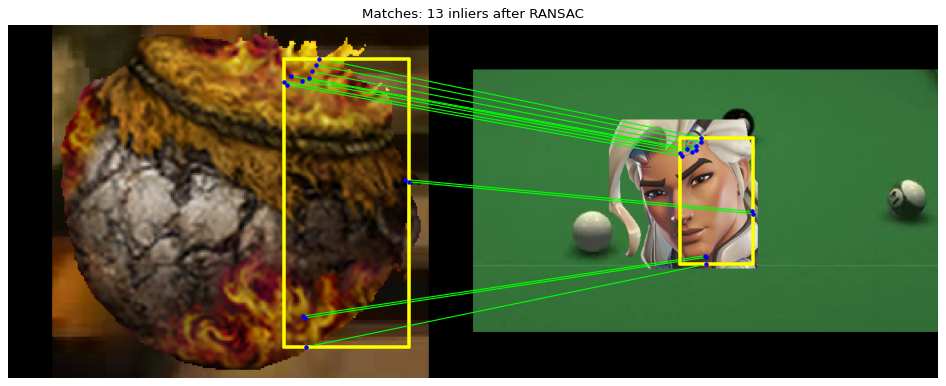
\includegraphics[width=0.7\textwidth]{ressources/false_positive_1.png}
    \caption{False Positive Example}
    \label{fig:false_positive_1}
\end{figure}

\subsection{Variant B}
In our new solution, we noticed that some icons contained semi-transparent
regions. When placed over a background, these pixels blended with the
background colors, creating a faint “merged” zone around and inside the icon.
This blending made the icon's edges less distinct and introduced background
information into what should be pure icon pixels. As a result, the network
could extract features from these shaded areas that are not native to the icon,
leading to confusing and noisy data and making it harder to learn accurate
features. To address this, we added a step in the data generation pipeline that
removes any pixel whose alpha value is below a chosen threshold, keeping only
fully opaque parts of the icon and ensuring a clean separation from the
background.
\begin{figure}[htbp]
    \centering
    \begin{minipage}{0.35\textwidth}
        \centering
        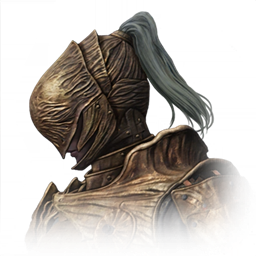
\includegraphics[width=\textwidth]{ressources/icon_4_original.png}
        \caption{Original Icon}
        \label{fig:original_icon}
    \end{minipage}
    \hfill
    \begin{minipage}{0.35\textwidth}
        \centering
        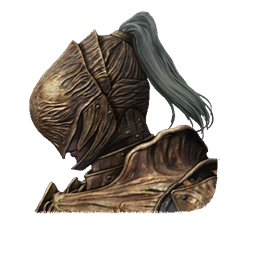
\includegraphics[width=\textwidth]{ressources/icon_4.png}
        \caption{Processed Icon}
        \label{fig:processed_icon}
    \end{minipage}
\end{figure}
Next we have added simple geometric transformations to our synthesis pipeline, where we would move the icon by random translations, to imitate the icon's position variability in real-world scenarios. And then we would keep the rest of the pipeline intact.
\begin{figure}[H]
    \centering
    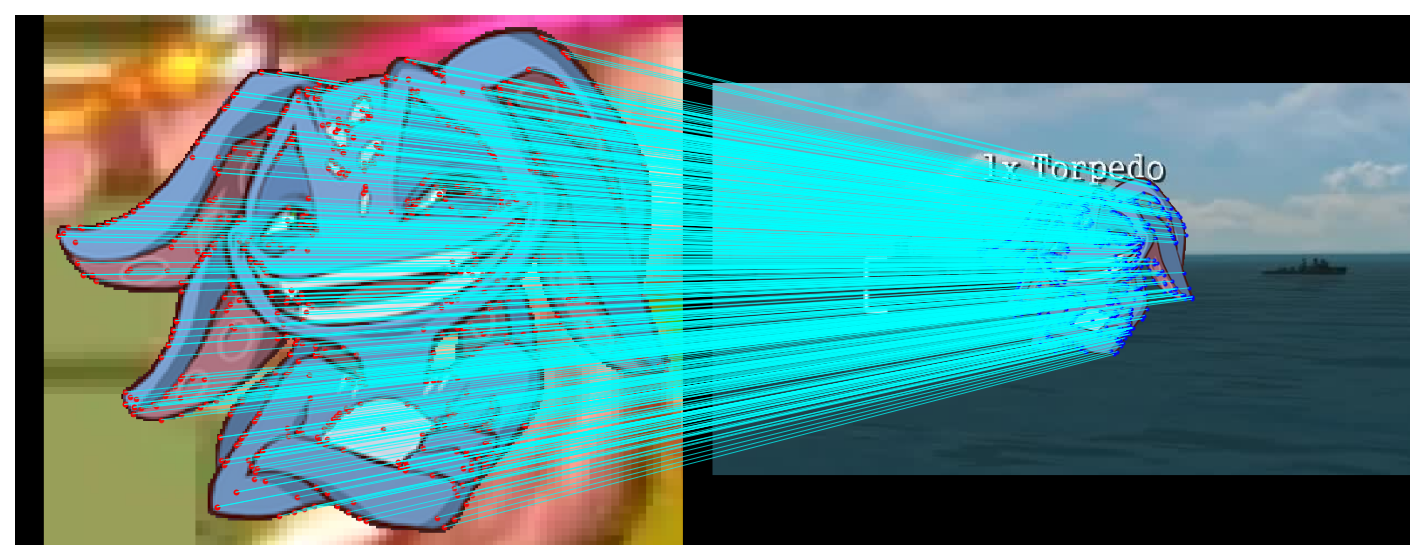
\includegraphics[width=0.8\textwidth]{ressources/image_3.png}
    \caption{Transformed Icon}
    \label{fig:transformed_icon}
\end{figure}
\subsubsection{Training Performance and Loss Analysis}

We conducted comprehensive training over 100,000 steps with multi-component
loss monitoring comprising coarse loss, fine loss, reliability loss, and total
loss, alongside validation evaluation every 1,000 steps. The training
demonstrated exceptional convergence across all metrics with a total loss
reduction of 78.1\% from 20.75 to 4.55.

\begin{figure}[H]
    \centering
    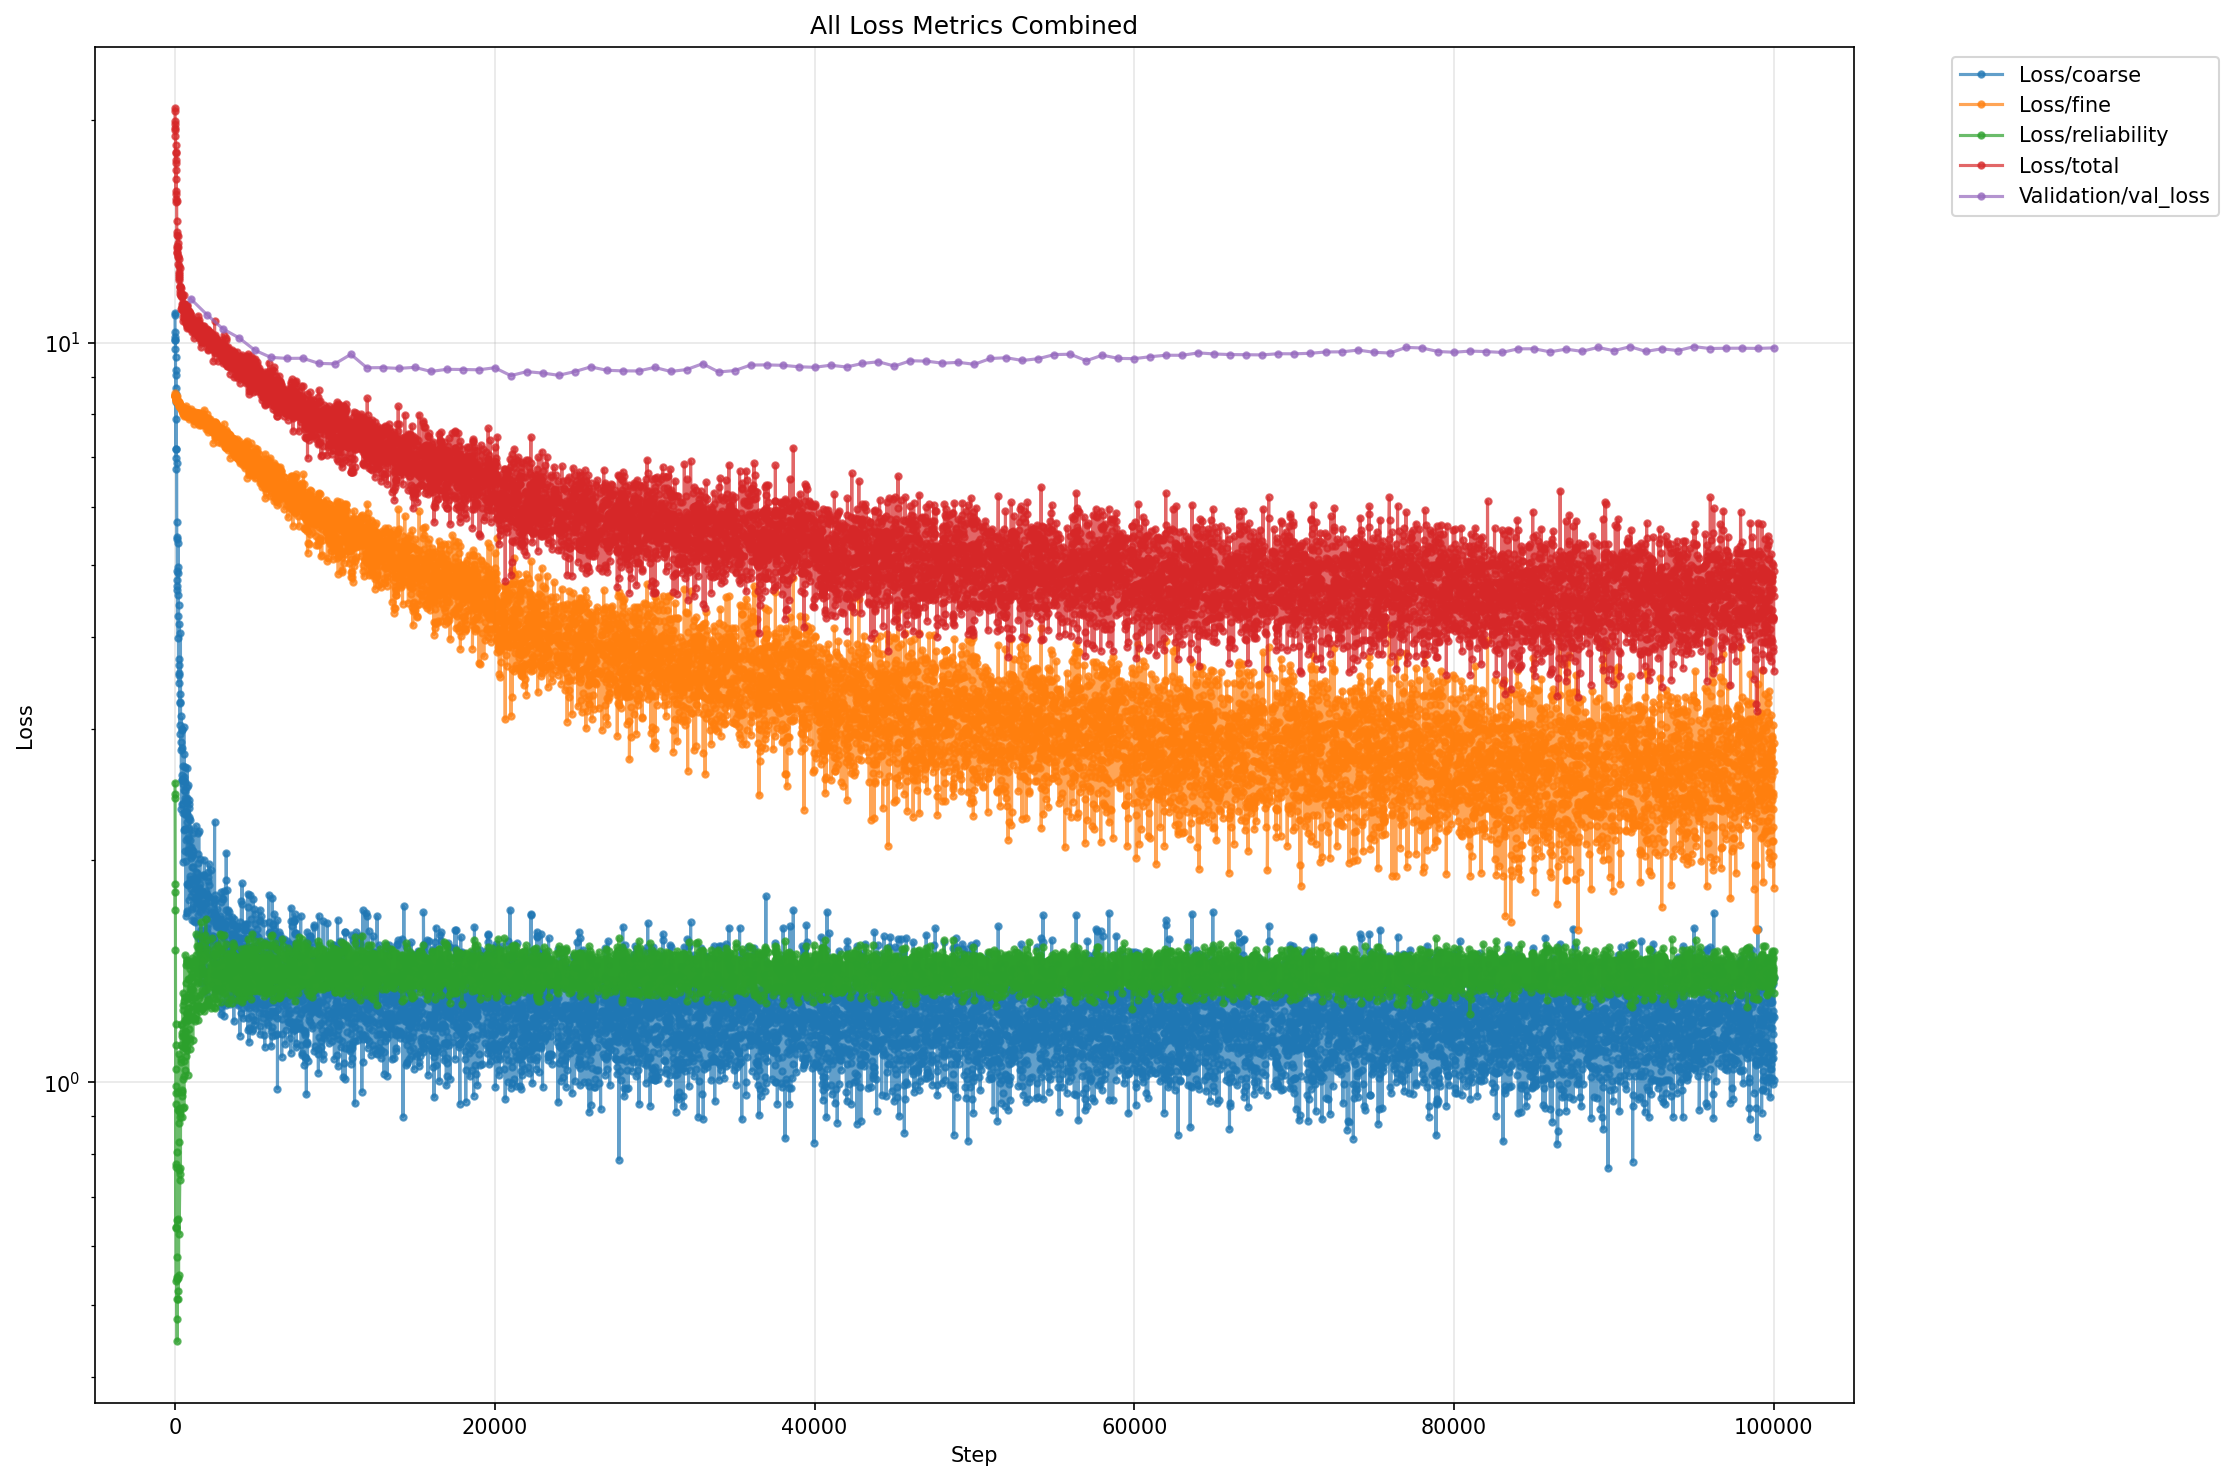
\includegraphics[width=0.8\textwidth]{ressources/loss_3.png}
    \caption{Loss Metrics}
    \label{fig:loss_components}
\end{figure}
The network exhibited rapid initial learning with total loss decreasing from 20.75 to approximately 8.0 within the first 20,000 steps. Component analysis revealed distinct optimization patterns: coarse loss achieved 88.8\% reduction (10.97→1.22), fine loss decreased by 69.1\% (8.51→2.63), and reliability loss improved by 45.4\% (2.54→1.39). This multi-faceted improvement indicates effective joint optimization across all network objectives (see Figure~\ref{fig:loss_components}).
\begin{figure}[H]
    \centering
    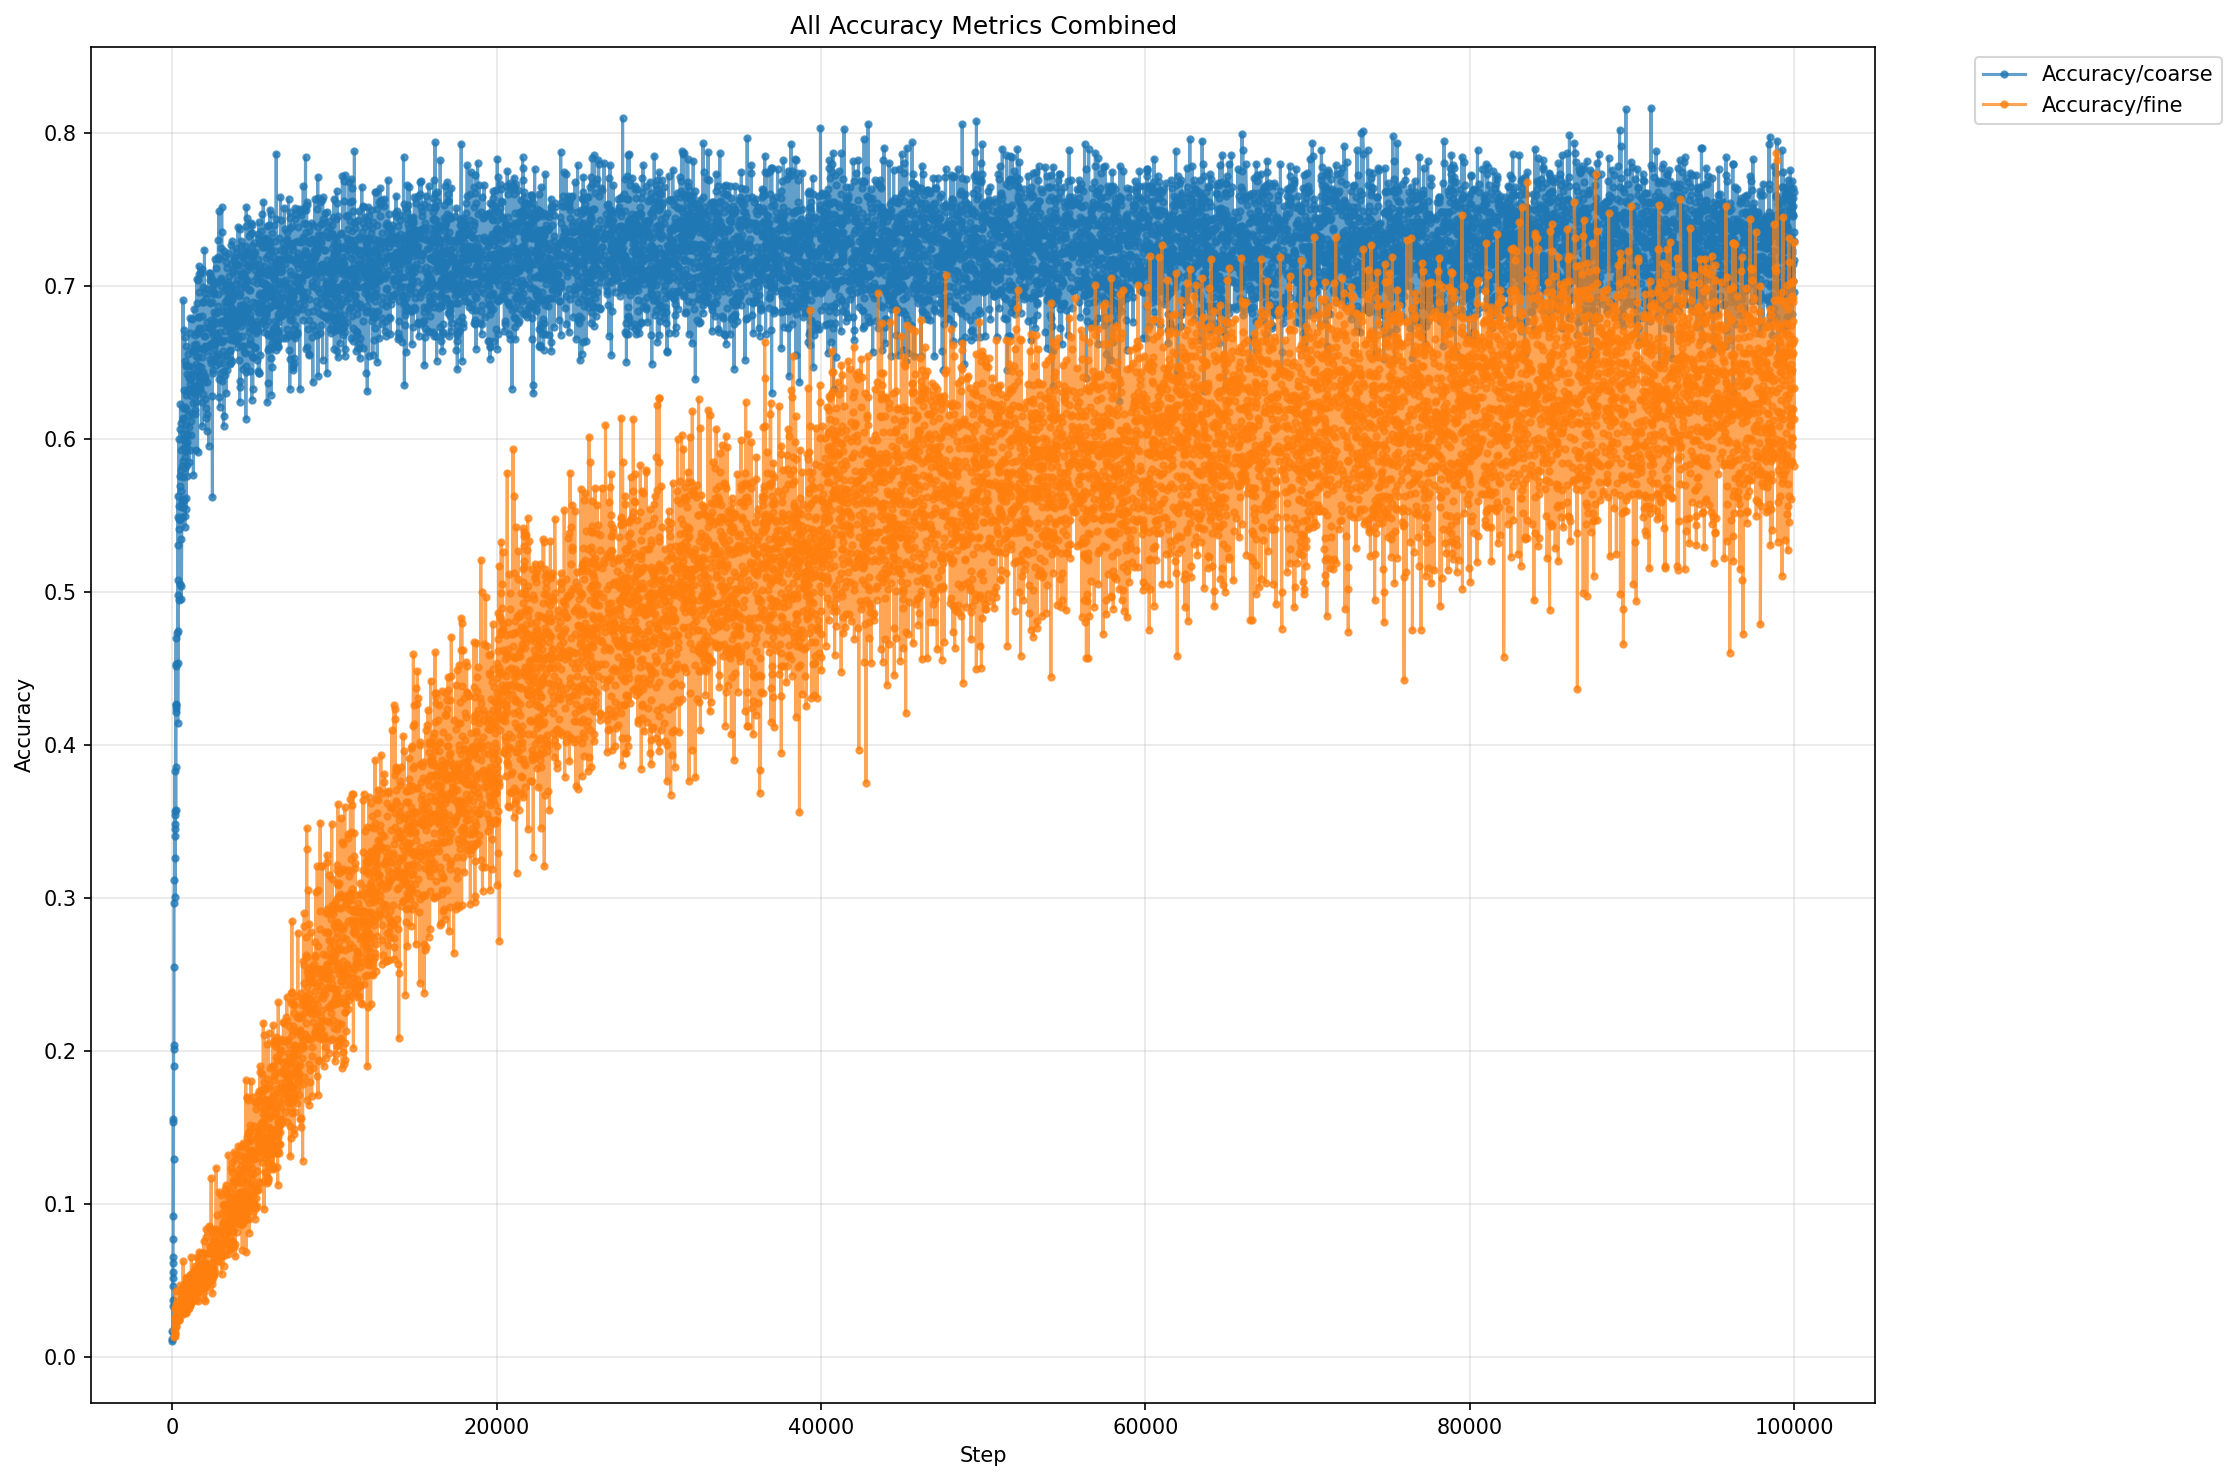
\includegraphics[width=0.8\textwidth]{ressources/accuracy_3.png}
    \caption{Accuracy Metrics}
    \label{fig:accuracy_metrics3}
\end{figure}

Accuracy metrics showed corresponding improvements, progressing from 1.01\% to
a peak of 81.65\% before stabilizing at 71.72\%. The validation loss trajectory
confirmed generalization capability, decreasing from 11.45 to 9.84 (14.1\%
improvement) with minimal overfitting indicators.
Figure~\ref{fig:accuracy_metrics3} illustrates the synchronized improvement
between accuracy and loss reduction throughout training.

The training exhibited three distinct phases: \textbf{rapid convergence} (0-20k
steps), \textbf{gradual refinement} (20k-70k steps), and \textbf{stabilization}
(70k-100k steps). All loss components demonstrated monotonic improvement with
minimal oscillations, indicating stable optimization dynamics. The final
validation loss of 9.84 and training accuracy of 71.72\% establish strong
baseline performance with excellent convergence properties.
\subsubsection{Confusion matrix}
\begin{figure}[H]
    \centering
    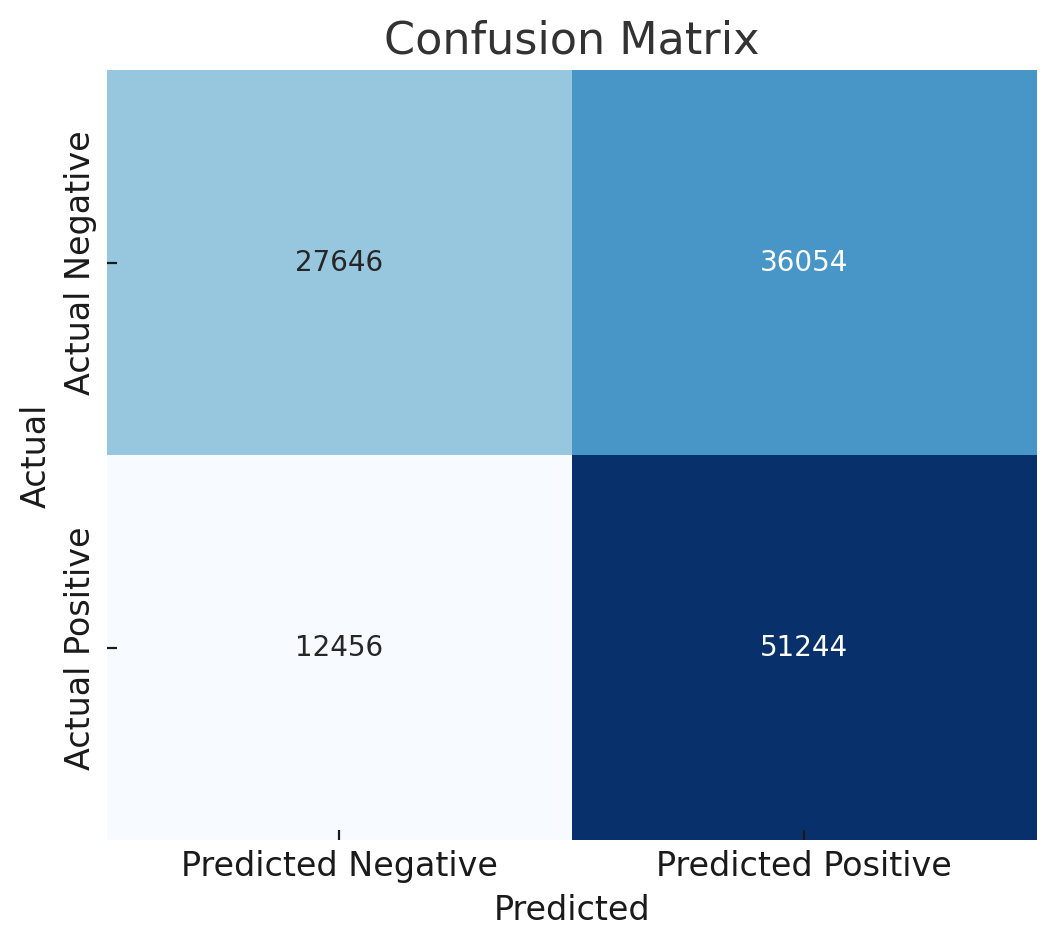
\includegraphics[width=0.7\textwidth]{ressources/confusion_matrix_3.png}
    \caption{Confusion matrix for variant B}
    \label{fig:confusion_matrix_3}
\end{figure}
\begin{itemize}
    \item \textbf{Accuracy: }0.619
    \item \textbf{Precision: }0.587
    \item \textbf{Recall: }0.804
    \item \textbf{F1 Score: }0.679
\end{itemize}
We could see that although the model can accurately detect the existence of keypoints, it still outputs an abnormally high false positive rate, which is a result of the overfitting of our model, and it not being able to generalize well to unseen data.
\subsubsection{Interpretation}
Although the training results show significant improvements in both loss and
accuracy metrics, the model still struggles with false positives, which is
result of the overfitting of our model. This could be proof that our choice of
teacher model is not optimal for this task, or that the model does not
generalize well to the target domain. To address this, we decided to explore an
alternative teacher model.
\subsection{Variant C}
We decided to return to our original approach and adopt SIFT as the teacher
method. Given that our SIFT-based solution already demonstrates strong
performance on the target task, it provides a robust and reliable supervisory
signal for training. In addition, we deliberately removed all forms of
filtering, such as RANSAC and masking, in order to increase the complexity of
the learning problem and reduce the risk of overfitting. This choice results in
a more raw and unfiltered dataset, encouraging the student model to generalize
more effectively under challenging conditions. For the supervision of our
detector, we rely on SIFT to extract interest points from both the reference
and target images. Rather than using the associated descriptors, we retain only
the keypoint locations, which are sufficient for our purpose. These coordinates
are then converted into ground-truth heatmaps by encoding each keypoint as a
binary mask. Formally, let $\mathcal{K} = \{(x_i, y_i)\}_{i=1}^{N}$ denote the
set of detected keypoints in an image of size $H \times W$. The ground-truth
heatmap $M \in \{0,1\}^{H \times W}$ is defined as
\begin{equation}
    M(x,y) =
    \begin{cases}
        1, & \text{if } (x,y) \in \mathcal{K}, \\
        0, & \text{otherwise}.
    \end{cases}
\end{equation}
This representation allows us to jointly supervise both the detector and the descriptor using ground-truth correspondences between image pairs, following the training paradigm introduced in XFeat~\cite{xfeat2023}.

\begin{figure}[H]
    \centering
    
\includegraphics[width=0.8\textwidth]{ressources/image_41_heatmap.png}
    \caption{SIFT Keypoint Heatmap}
\end{figure}
Then we use These keypoints from both images to generate ground-truth correspondences.
\begin{figure}[H]
    \centering
    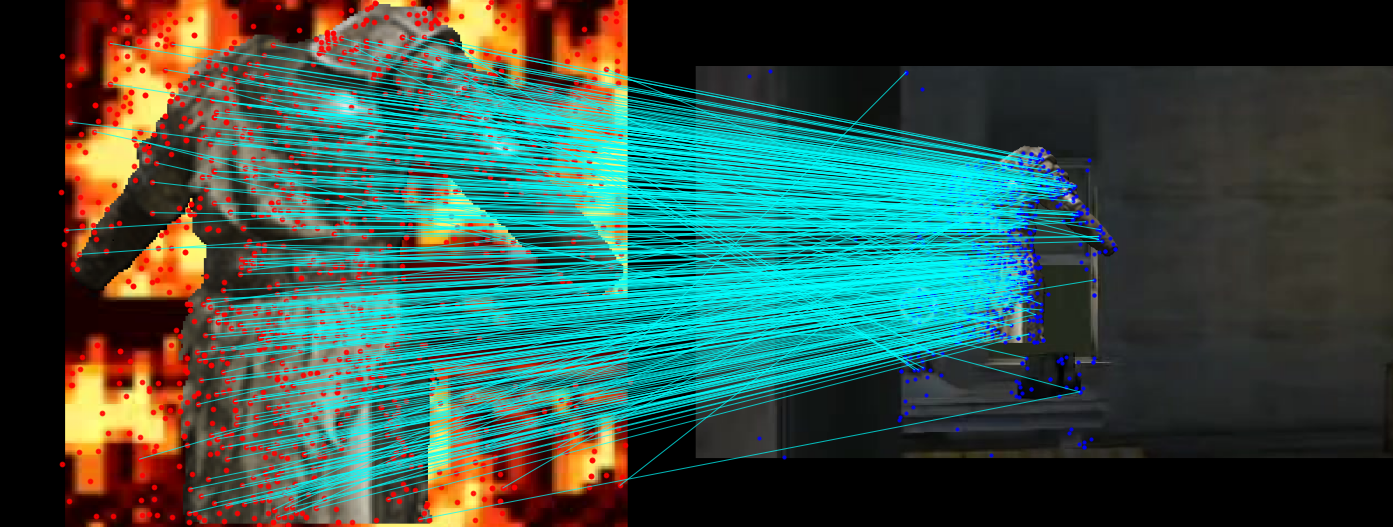
\includegraphics[width=0.8\textwidth]{ressources/image_41.png}
    \caption{SIFT Keypoint Detection Example}
    \label{fig:sift_example}
\end{figure}
\subsubsection{Training Performance and Loss Analysis}
We trained for \(\sim145\text{k}\) steps (0–144{,}688) with multi-component
loss monitoring (coarse, fine, reliability, and total) and validation every
1{,}000 steps. Optimization was decisive: the \textbf{total loss} fell by
\(\mathbf{81.65\%}\) from \(\mathbf{23.36}\rightarrow\mathbf{4.29}\), with a
rapid \(\mathbf{78.24\%}\) drop by \(\sim\)20k steps \((23.36\rightarrow
5.08)\). Component trends showed coordinated progress
(Fig.~\ref{fig:loss_components}): \textbf{coarse loss} improved
\(\mathbf{83.86\%}\) \((13.47\rightarrow 2.17)\), \textbf{fine loss}
\(\mathbf{81.51\%}\) \((8.64\rightarrow 1.60)\), and \textbf{reliability loss}
decreased more moderately by \(\mathbf{58.79\%}\) \((2.49\rightarrow 1.03)\).
Minima were reached early for reliability \((\mathbf{0.152}\ \text{at }
\mathbf{step\ 146})\) and coarse \((\mathbf{0.923}\ \text{at } \mathbf{step\
    6{,}276})\), with later troughs for fine \((\mathbf{1.003}\ \text{at }
\mathbf{step\ 129{,}639})\) and total \((\mathbf{3.718}\ \text{at }
\mathbf{step\ 129{,}639})\), consistent with a fast coarse/reliability
stabilization followed by slower fine-grained refinement.

\begin{figure}[H]
    \centering
    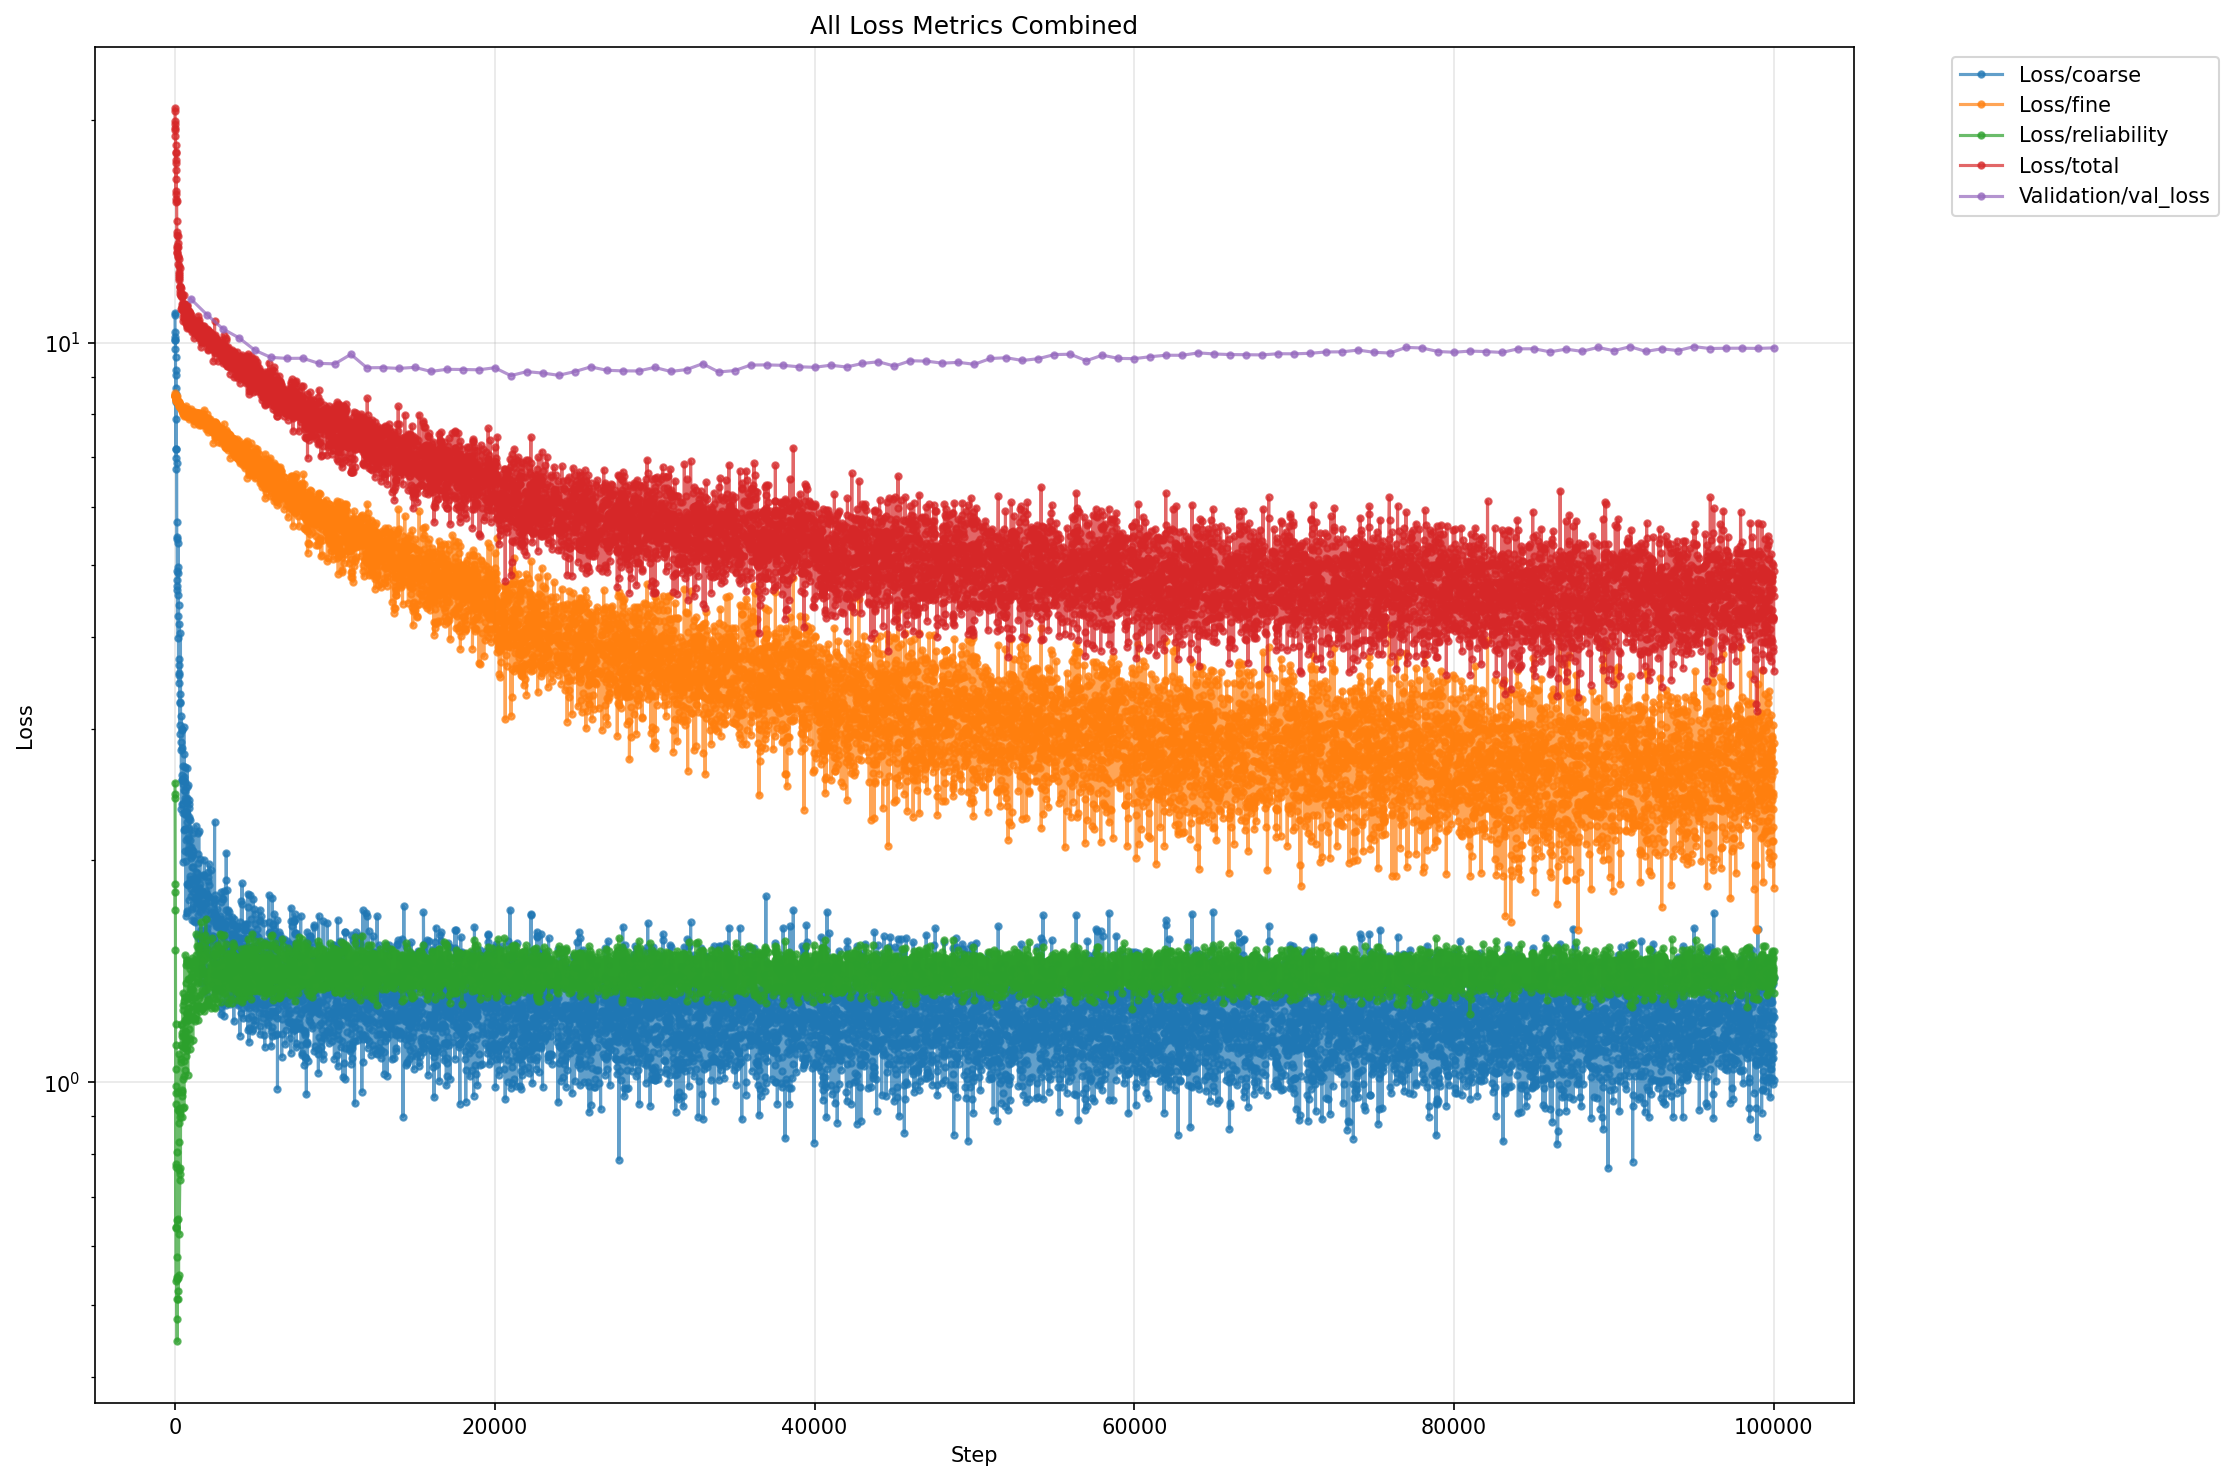
\includegraphics[width=0.8\textwidth]{ressources/loss_3.png}
    \caption{Loss Metrics}
    \label{fig:loss_components}
\end{figure}
Accuracy evolved in step with losses but with distinct behaviors across heads (Fig.~\ref{fig:accuracy_metrics3}). \textbf{Fine accuracy} peaked at \(\mathbf{100\%}\) (step \(\sim\)1{,}267) and stabilized at a strong late-training band (mean of last 10\% \(\approx \mathbf{78.62\%}\); final reading \(\mathbf{64.00\%}\)), indicating high-fidelity fine predictions despite endpoint variance. \textbf{Coarse accuracy} peaked at \(\mathbf{70.37\%}\) (step \(\sim\)63{,}515) but drifted downward thereafter (last-10\% mean \(\approx \mathbf{21.06\%}\); final \(\mathbf{15.14\%}\)), suggesting increasing sensitivity or over-confidence at the coarse stage as training progressed.

\begin{figure}[H]
    \centering
    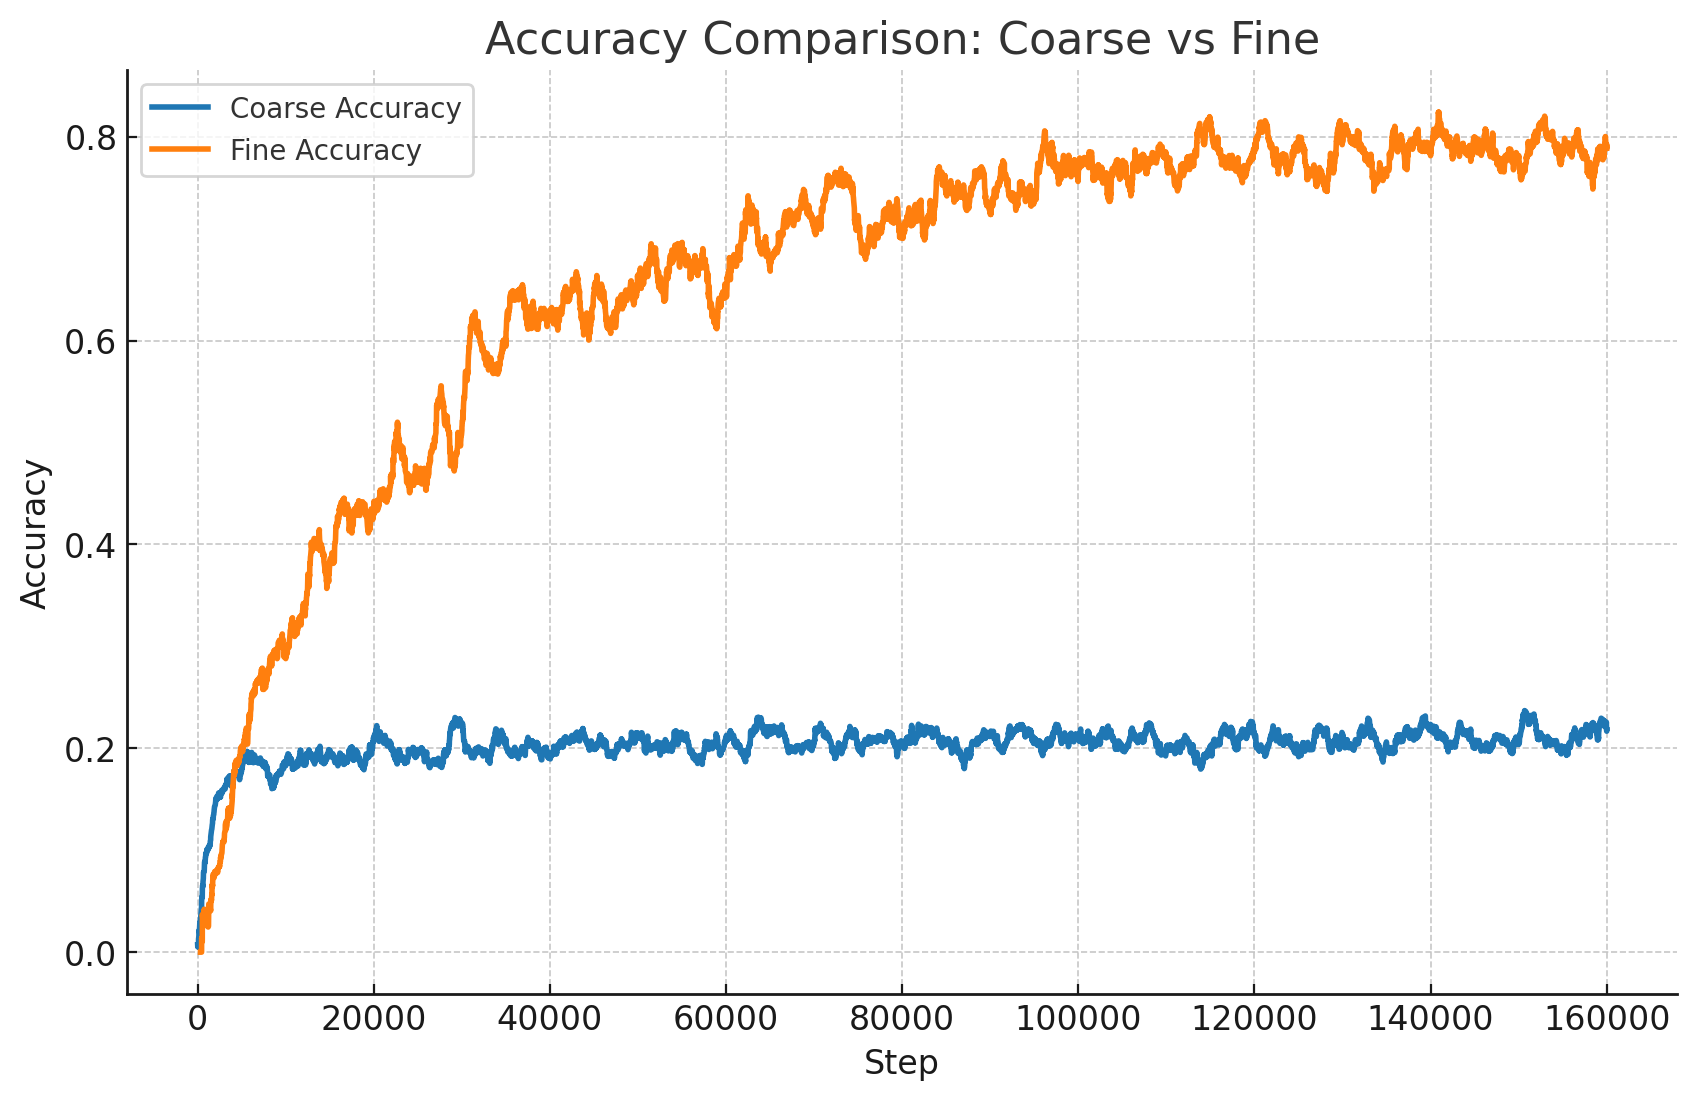
\includegraphics[width=0.8\textwidth]{ressources/accuracy_4.png}
    \caption{Accuracy Metrics}
    \label{fig:accuracy_metrics3}
\end{figure}

The validation trajectory clarifies generalization. It improved early
\((\mathbf{11.25}\ \text{at }999 \rightarrow \mathbf{10.20}\ \text{by
}\sim\!20\text{k}; \text{best } \mathbf{8.12}\ \text{at }\sim\!8\text{k})\),
then rose steadily to \(\mathbf{17.63}\) by the end, signaling late overfitting
despite continued training-loss gains. Overall, training exhibited three
phases: \textbf{rapid convergence} (0–20k), \textbf{gradual refinement}
(20k–100k), and a \textbf{late drift} (>100k) where optimization continues but
validation degrades. As a baseline, this run demonstrates excellent
optimization and mature fine-level accuracy; for deployment, prefer early
stopping around the validation minimum (\(\sim\)8–20k) or strengthen
regularization (e.g., heavier augmentation, dropout/weight decay, stochastic
depth) to preserve the early generalization peak while maintaining the gains in
fine accuracy.

\subsubsection{Confusion matrix}
\begin{figure}[H]
    \centering
    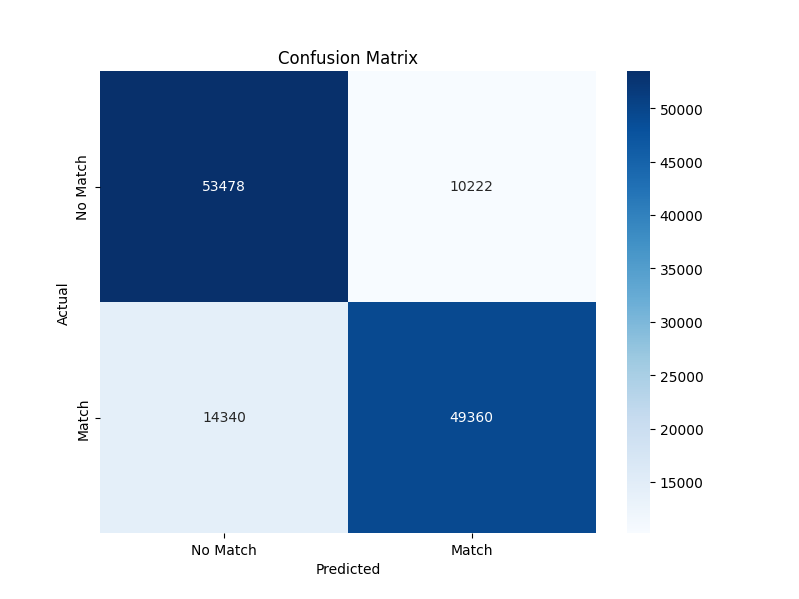
\includegraphics[width=0.8\textwidth]{ressources/cm_L_10.png}
    \caption{Confusion matrix for variant C}
    \label{fig:confusion_matrix_4}
\end{figure}
The new formula shows better promising results, the number of false positives has decreased significantly, increasing the overall precision of the model. With these results, this remains our best performing model so far, and we can see that the model is able to learn the keypoints and descriptors from the SIFT teacher model, and generalize well to unseen data.



% ------------------------------------------------------------
\chapter{Results \& Analysis}
\section{Analysis \& Discussion}
\subsection{Comparative Analysis}
In order to properly evaluate the performance of our model, we needed a
baseline model to compare against. We chose the original pretrained XFeat
models~\cite{xfeat_github} as they are we try to optimize for our target use
case. The evaluation test yielded the following results:
\begin{figure}[H]
    \centering
    \includegraphics[width=0.6\textwidth]{ressources/xfeat_cm.png}
    \caption{Evaluation results comparison}
    \label{fig:evaluation_results}
\end{figure}
\begin{table}[H]
    \centering
    \renewcommand{\arraystretch}{1.2}
    \begin{tabular}{lcccc}
        \toprule
        \textbf{Class}        & \textbf{Precision} & \textbf{Recall} & \textbf{F1-score} & \textbf{Support} \\
        \midrule
        No Match              & 0.73               & 0.87            & 0.79              & 63,700           \\
        Match                 & 0.84               & 0.67            & 0.75              & 63,700           \\
        \midrule
        \textbf{Accuracy}     &                    &                 & 0.77              & 127,400          \\
        \textbf{Macro Avg}    & 0.78               & 0.77            & 0.77              & 127,400          \\
        \textbf{Weighted Avg} & 0.78               & 0.77            & 0.77              & 127,400          \\
        \bottomrule
    \end{tabular}
    \caption{Classification report on XFeat.}
    \label{tab:classification_report}
\end{table}
Compared to our models' performance:
\begin{table}[H]
    \centering
    \renewcommand{\arraystretch}{1.2}
    \begin{tabular}{lcccc}
        \toprule
        \textbf{Class}        & \textbf{Precision} & \textbf{Recall} & \textbf{F1-score} & \textbf{Support} \\
        \midrule
        No Match              & 0.79               & 0.84            & 0.81              & 63,700           \\
        Match                 & 0.83               & 0.77            & 0.80              & 63,700           \\
        \midrule
        \textbf{Accuracy}     &                    &                 & 0.81              & 127,400          \\
        \textbf{Macro Avg}    & 0.81               & 0.81            & 0.81              & 127,400          \\
        \textbf{Weighted Avg} & 0.81               & 0.81            & 0.81              & 127,400          \\
        \bottomrule
    \end{tabular}
    \caption{Classification report with precision, recall, F1-score, and support for the two classes.}
    \label{tab:classification_report2}
\end{table}
Overall, the model achieved an accuracy of \textbf{75\%}. However, it performed better at identifying ``No Match'' pairs than at detecting all the ``Match'' pairs. The model is very cautious about calling something a ``Match''. When it does, it is usually correct, but it misses many true matches.

\subsubsection*{Detailed Breakdown}

Here is what each term means in the context of the results:

\begin{itemize}
    \item \textbf{Precision:} Of all the times the model predicted a certain class, how often was it correct?
          \begin{itemize}
              \item \textbf{No Match (0.79):} When the model predicted ``No Match'', it was correct only 79\% of the time.
              \item \textbf{Match (0.83):} When the model predicted ``Match'', it was correct 83\% of the time. This is high and means the model produces fewer false positives.
          \end{itemize}

    \item \textbf{Recall:} Of all the actual instances of a class, how many did the model correctly identify?
          \begin{itemize}
              \item \textbf{No Match (0.84):} The model correctly identified 84\% of all actual ``No Match'' pairs.
              \item \textbf{Match (0.77):} The model only found 77\% of all the true ``Match'' pairs. This means it missed 23\% of them, leading to many false negatives.
          \end{itemize}

    \item \textbf{F1-Score:} The harmonic mean of Precision and Recall. It balances the trade-off between the two. The model has a decent F1-score for both classes, but the lower recall for ``Match'' reduces its value.

    \item \textbf{Support:} The number of actual occurrences of each class in the dataset.
\end{itemize}

\subsubsection*{Averages}

\begin{itemize}
    \item \textbf{Accuracy (0.81):} The overall percentage of correct predictions (81\% of 63,700 pairs).
    \item \textbf{Macro Avg (0.81, 0.81, 0.81):} The unweighted average across both classes, treating ``Match'' and ``No Match'' equally.
    \item \textbf{Weighted Avg (0.81, 0.81, 0.81):} The average weighted by the number of samples. Since there are more ``Match'' pairs, the average is biased towards their scores.
\end{itemize}

\subsubsection*{In Simple Terms}

The model is very conservative, it avoids calling something a match unless it
is very certain.

\begin{itemize}
    \item \textbf{Good news:} When it says ``Match'', we can trust it (81\% precision).
    \item \textbf{Bad news:} It fails to identify a quarter of the actual matches (77\% recall), classifying them instead as ``No Match''.
\end{itemize}
\subsection{Trade-offs: Speed vs. Accuracy}
\begin{tabular}{l r r r r r r r r}
\toprule
Method    & Extraction(s) & Speedup & Matching(s) & Speedup & Total(s) & Speedup & Matches & Matches/s \\
\midrule
SIFT-CPU  & 0.1420 & 1.0  & 0.0024 & 0.63 & 0.1443 & 1.0  & 579  & 244319 \\
XFeat-GPU & 0.0117 & 12.1 & 0.0015 & 1.0  & 0.0132 & 10.9 & 256  & 19394  \\
XFeat-CPU & 0.0110 & 12.9 & 0.0006 & 2.5  & 0.0116 & 12.4 & 256  & 220690 \\
\bottomrule
\end{tabular}


\vspace{1em}

The results highlight a pronounced contrast between SIFT and XFeat in terms of computational efficiency. 
XFeat demonstrates a substantial speed advantage, outperforming SIFT across extraction, matching, and total runtime.
Notably, XFeat achieves these gains even on the CPU, underscoring its efficiency and making it a strong candidate 
for deployment in environments where GPU resources are limited or unavailable. 
However, this gain in speed comes at the cost of accuracy. While XFeat delivers results an order of magnitude faster, 
its number of matches is significantly lower than SIFT's, which translates into reduced reliability in many 
feature-matching tasks. SIFT, despite being slower, provides at least 15\% higher accuracy, which can be 
critical in applications where precision is more important than raw throughput. 
Overall, these findings illustrate the fundamental trade-off between speed and accuracy: XFeat offers 
exceptional performance efficiency, while SIFT remains more robust in terms of match quality.

\subsection{Visual Results on Gaming Footage}

\section{Computational Efficiency}
\subsection{FPS and Latency Benchmarks}
\subsection{Memory and CPU Usage Profiles}


% ------------------------------------------------------------
\chapter{Conclusion and Future Work}
\section{Summary of Contributions}
\section{Limitations}
\subsection{Domain Generalization}
\subsection{Extreme Low-Light or High-Motion Scenes}

\section{Future Work}
\subsection{Hardware-Specific Optimizations (e.g., ARM CPU Tuning)}
\subsection{Real-Time Deployment on End-User Devices}

% ------------------------------------------------------------
\chapter{Appendices}
\section{Additional Figures}
\section{Code Snippets}
\section{Hyperparameter Tables}
\section{Hardware Specifications}
% ------------------------------------------------------------

% Add bibliography here
\bibliographystyle{plain}  % or another style: ieeetr, apalike, etc.
\bibliography{ref}         % filename without .bib extension

\end{document}
